\chapter{Random Variables}

\section{Intro}


\begin{enumerate}
    \item A random variable is a numerical outcome of a random process.
    A random variable assigns a number to each possible outcome of a random experiment.
    \hfill \cite{common/online/chatgpt}

    \item An intuitive definition of a random variable or random quantity is a variable for which the value or outcome is unknown and for which the outcome is influenced by some form of random phenomenon.
    \hfill \cite{statistics/book/Statistics-for-Data-Scientists/Maurits-Kaptein}

    \item Why is it called "random"?
    Because the value it takes depends on chance.
    You don’t know the outcome in advance, but you know the possible values and can assign probabilities to them.
    \hfill \cite{common/online/chatgpt}

    \item This allows us to extend our theory on probability to other types of data without restricting it to specific events (i.e., binary data).
    \hfill \cite{statistics/book/Statistics-for-Data-Scientists/Maurits-Kaptein}

    \item The probability sampling approach makes the variable of interest a random variable, as the sampling approach is here the random phenomenon.
    \hfill \cite{statistics/book/Statistics-for-Data-Scientists/Maurits-Kaptein}

    \item A realization or an outcome of the random variable is then indicated by the same, but lower case, letter.
    \hfill \cite{statistics/book/Statistics-for-Data-Scientists/Maurits-Kaptein}

    \item a random variable may be seen as a variable that can in principle be equal to any of the values in the population, and after probability sampling the outcome(s) will become known.
    \hfill \cite{statistics/book/Statistics-for-Data-Scientists/Maurits-Kaptein}

    \item Types of Random Variables:
    \hfill \cite{common/online/chatgpt}
    \begin{enumerate}
        \item Discrete Random Variable:
        \hfill \cite{common/online/chatgpt}
        \begin{enumerate}
            \item Takes countable values (e.g., 0, 1, 2, 3…)
            \hfill \cite{common/online/chatgpt}

            \item Examples: number of heads in 10 coin tosses, number of emails received
            \hfill \cite{common/online/chatgpt}
        \end{enumerate}

        \item Continuous Random Variable
        \hfill \cite{common/online/chatgpt}
        \begin{enumerate}
            \item Takes uncountably many values in an interval (e.g., any real number)
            \hfill \cite{common/online/chatgpt}

            \item Examples: height of a person, temperature, time taken to run a race
            \hfill \cite{common/online/chatgpt}
        \end{enumerate}
    \end{enumerate}

    \item Notation:
    \begin{enumerate}
        \item Random variables are often written as capital letters like $X, Y, Z$
        \hfill \cite{common/online/chatgpt}

        \item Their values are written in lowercase, e.g., $X=x$
        \hfill \cite{common/online/chatgpt}
    \end{enumerate}

    \item The \textbf{probability function} $P(X \leq x)$ is a general concept and can be used for any random variable.
    \hfill \cite{statistics/book/Statistics-for-Data-Scientists/Maurits-Kaptein}

    \item The PMF for a discrete random variable is the equivalent of the PDF for a continuous random variable.
    \hfill \cite{statistics/book/Statistics-for-Data-Scientists/Maurits-Kaptein}

    \item The probability $P(X \leq x)$ is also referred to as the \textbf{distribution function} obtained in $x$ and it is denoted by $F(x) = P(X \leq x)$.
    Thus every random variable $X$ has a distribution function $F$ through $F(x) = P(X \leq x)$, but also every distribution function $F$ has a random variable $X$, namely the random variable $X$ that makes $P(X \leq x) = F(x)$.
    Thus the two concepts are directly related to each other and we then typically say that $X$ is distributed according to $F$, i.e., \colorbox{yellow}{$X \sim F$}.
    \hfill \cite{statistics/book/Statistics-for-Data-Scientists/Maurits-Kaptein}

    \item Each distribution function $F$ typically satisfies three conditions:
    \begin{enumerate}
        \item When the value $x$ increases to infinity, the distribution function becomes equal to one, i.e., $\lim _{x\to \infty} F(x) = 1$.
        \hfill \cite{statistics/book/Statistics-for-Data-Scientists/Maurits-Kaptein}

        \item When the value $x$ decreases to minus infinity the distribution function becomes equal to zero, i.e., $\lim _{x\to -\infty} F(x) = 0$.
        \hfill \cite{statistics/book/Statistics-for-Data-Scientists/Maurits-Kaptein}

        \item The distribution function is a non-decreasing function, i.e., $F(x_1) \leq F(x_2)$ when $x_1 \leq x_2$.
        \hfill \cite{statistics/book/Statistics-for-Data-Scientists/Maurits-Kaptein}
    \end{enumerate}


    \item Data points that are drawn independently from the same distribution ($D$ OR $D(\cdots)$) are said to be \textbf{independent and identically distributed}, which is often abbreviated to i.i.d. (denoted by $x \sim D$ OR $x \sim D(\cdots)$)
    \hfill \cite{ml/book/Pattern-Recognition-And-Machine-Learning/Christopher-M-Bishop}

    \item We consider multivariate random variables $X$ as a finite vector of univariate random variables $\begin{bmatrix}X_1 & \cdots & X_D\end{bmatrix}^\top$. 
    \hfill \cite{mfml/book/mml/Deisenroth-Faisal-Ong}
\end{enumerate}








\section{Joint Distribution Function ($F _{X Y}$, $F _{X_1 X_2 ... X _K} $)}

\begin{enumerate}
    \item The joint distribution function contains all the information on how the random variables are related to each other, i.e., how the random variables are dependent on each other.
    \hfill \cite{statistics/book/Statistics-for-Data-Scientists/Maurits-Kaptein}

    \item If one variable increases and the other variable also increases (on average) or if one variable increases while the other variable decreases (on average) they are said to \textbf{co-relate}.
    \hfill \cite{statistics/book/Statistics-for-Data-Scientists/Maurits-Kaptein}

    \item We say that random variables $X$ and $Y$ have a joint distribution function $F _{X Y}$ if the probability that $X$ is observed in the interval $(-\infty, x]$ and the probability that $Y$ is observed in the interval $(-\infty, y]$ is given by the function $F _{X Y}$ , i.e., $P (X \leq x, Y \leq y) = F _{X Y} (x, y)$.
    The joint distribution function of two random variables is also called a \textbf{bivariate distribution function}.
    \hfill \cite{statistics/book/Statistics-for-Data-Scientists/Maurits-Kaptein}

    \item the joint distribution function of $K$ random variables $X_1, X_2, \cdots , X_K$ , i.e,
    $F _{X_1 X_2 \cdots X _K} = P(X_1 \leq x_1, X_2 \leq x_2, \cdots , X_K \leq x_K )$
    is called a \textbf{multivariate distribution function}.
    \hfill \cite{statistics/book/Statistics-for-Data-Scientists/Maurits-Kaptein}
\end{enumerate}



\subsection{Independence of Random Variables}

\begin{enumerate}
    \item Two random variables $X$ and $Y$ are called independent when the bivariate distribution function is equal to the product of the marginal distribution functions.
    \hfill \cite{statistics/book/Statistics-for-Data-Scientists/Maurits-Kaptein}

    \item independence of $X$ and $Y$ holds when $F _{X Y} (x, y) = F_X (x)F_Y (y)$ for all $(x, y) \in \mbbR \times \mbbR$, with $F _X$ the CDF of $X$ and $F_Y$ the CDF of $Y$
    \hfill \cite{statistics/book/Statistics-for-Data-Scientists/Maurits-Kaptein}

    \item The random variables $X_1 , X_2, \cdots , X_K$ are called \textbf{mutually independent} when the joint distribution function is the product of the marginal distribution functions, i.e.,
    \hfill \cite{statistics/book/Statistics-for-Data-Scientists/Maurits-Kaptein}
    \\
    $F _{X_1 X_2 \cdots X_K} (x_1, x_2, \cdots , x_K ) = F _{X_1} (x_1)F_{X_2} (x_2) \cdots F_{X_K} (x_K )$ for all $x_k \in \mbbR$.
    \hfill \cite{statistics/book/Statistics-for-Data-Scientists/Maurits-Kaptein}

    \item If in case we assume that all distribution functions are identical, i.e., $F_ {X_1} (x) = F _{X_2} (x) = \cdots = F _{X_K} (x) = F(x)$ for all $x$, then we have the concept of $X_1 , X_2, \cdots , X_K$ being i.i.d. with distribution function $F$
    \hfill \cite{statistics/book/Statistics-for-Data-Scientists/Maurits-Kaptein}

    \item The random variables $X$ and $Y$ are called \textbf{dependent} when they are not independent.
    \hfill \cite{statistics/book/Statistics-for-Data-Scientists/Maurits-Kaptein}

    \item we may have that $X$ and $Y$ , $X$ and $Z$ , and $Y$ and $Z$ are \textbf{(pairwise) independent}, but $X$ , $Y$ , and $Z$ are not mutually independent.
    Thus we may have $F _{X Y} (x, y) = F _X (x)F_Y (y)$, $F _{X Z} (x, z) = F_X (x)F_Z (z)$, and $F_{Y Z} (y, z) = F_Y (y)F_Z (z)$ for all $x$, $y$, and $z$, but we may not have $F _{X Y Z} (x, y, z) = F_X (x)F_Y (y)F_Z (z)$ for all $x$, $y$, and $z$.
    \hfill \cite{statistics/book/Statistics-for-Data-Scientists/Maurits-Kaptein}

    \item Pairwise independence is thus \textbf{weaker} than mutual independence.
    When we talk about independence among multiple random variables we mean mutual independence.
    \hfill \cite{statistics/book/Statistics-for-Data-Scientists/Maurits-Kaptein}

    \item 2 types of dependencies/ independencies:
    \begin{enumerate}
        \item Variables of same unit, ($X_i, Y_i, \cdots$), where $i$ is unit.
        Example: height \& weight of same person

        \item Different Units of sample/ population.
        Example: heights of siblings, hair color of a family, etc
    \end{enumerate}
\end{enumerate}










\section{Discrete Functions}

\subsection{Univariate PMF ($f(x_k) = p_k = P(X = x_k)$)}

\begin{enumerate}
    \item Discrete does not always mean that we observe values in $\mathbb{N}$.
    For instance, grades on a data science test may take values in $\dCurlyBrac{1, 1.5, 2.0, 2.5, \cdots , 9.0, 9.5, 10}$.
    Thus, it would be more rigorous to say that a discrete random variable $X$ takes its values in the set $\dCurlyBrac{x_0, x_1, x_2, \cdots , x _k , \cdots}$, with $x _k$ an element of the real line $(x _k \in \mbbR)$ and with an ordering of the values $x_0 < x_1 < x_2 < \cdots$ .
    However, in many practical settings we can map this set to a subset of $\mathbb{N}$ or to the whole set $\mathbb{N}$.
    \hfill \cite{statistics/book/Statistics-for-Data-Scientists/Maurits-Kaptein}

    \item For discrete random variables we can define $p _k = P(X = k)$ as the probability of observing the outcome $k$.
    \hfill \cite{statistics/book/Statistics-for-Data-Scientists/Maurits-Kaptein}

    \item This is referred to as the probability mass function (PMF) if the probabilities $p _k$ satisfy two conditions.
    \hfill \cite{statistics/book/Statistics-for-Data-Scientists/Maurits-Kaptein}
    \begin{enumerate}
        \item all probabilities $p _k$ should be nonnegative ( $p _k \geq 0, \forall\ k$)
        \hfill \cite{statistics/book/Statistics-for-Data-Scientists/Maurits-Kaptein}

        \item probabilities need to add up to one, i.e., $\dsum^{\infty}_{k=0} p _k = 1$
        \hfill \cite{statistics/book/Statistics-for-Data-Scientists/Maurits-Kaptein}
    \end{enumerate}
\end{enumerate}


\subsection{CDF of Univariate PMF ($F(x)$)}

\begin{enumerate}
    \item The distribution function or cumulative density function (CDF) for a discrete random variable $X$ is now given by \colorbox{yellow}{$F(x) = P(X \leq x) = \dsum^{x}_ {k=0} f (k)$}.
    \hfill \cite{statistics/book/Statistics-for-Data-Scientists/Maurits-Kaptein}

    \item If the set is $\dCurlyBrac{x_0, x_1, x_2, \cdots , x _k , \cdots}$, with $x_0 < x_1 < x_2 < \cdots$ , then the CDF is defined as \colorbox{yellow}{$F(x) =\dsum^{m_x} _{k=0} f (x _k )$}, with $m _x$ the largest value for $k$ that satisfies $x_ k \leq x$.
    \hfill \cite{statistics/book/Statistics-for-Data-Scientists/Maurits-Kaptein}
\end{enumerate}




\subsection{Bivariate Joint PMF ($f _{X Y} (x, y) = P(X = x, Y = y)$)}

\begin{enumerate}
    \item If $X$ and $Y$ are both discrete random variables, than the joint probability mass function (PMF) is $f _{X Y} (x, y) = P(X = x, Y = y)$, $x, y\in \mathbb{N}$
    \hfill \cite{statistics/book/Statistics-for-Data-Scientists/Maurits-Kaptein}

    \item Some or many combinations of pairs $(x, y)$ may not occur, which implies that the probability for these values is zero, i.e., $f _{X Y} (x, y) = 0$.
    \hfill \cite{statistics/book/Statistics-for-Data-Scientists/Maurits-Kaptein}

    \item
    $
        \dsum _{(x,y)\in \mathbb{N}\times \mathbb{N}} f _{X Y} (x, y)
        = \dsum^\infty _{x=0} \dsum^\infty _{y=0} f _{X Y} (x, y)
        = \dsum^\infty _{y=0} \dsum^\infty _{x=0} f _{X Y} (x, y)
        = 1
    $
    \hfill \cite{statistics/book/Statistics-for-Data-Scientists/Maurits-Kaptein}

    \item Marginal PMFs:
    \begin{enumerate}
        \item marginal PMF of $X$: $f _X (y) = \dsum^\infty _{y=0} f _{X Y} (x, y)$
        \hfill \cite{statistics/book/Statistics-for-Data-Scientists/Maurits-Kaptein}

        \item marginal PMF of $Y$: $f _Y (y) = \dsum^\infty _{x=0} f _{X Y} (x, y)$
        \hfill \cite{statistics/book/Statistics-for-Data-Scientists/Maurits-Kaptein}
    \end{enumerate}

    \item When the random variables $X$ and $Y$ are \textbf{independent}, $f _{X Y} (x, y) = f_X (x) f_Y (y)$.
    \hfill \cite{statistics/book/Statistics-for-Data-Scientists/Maurits-Kaptein}
    \\
    \textbf{Proof}:
    \\
    $
        \begin{aligned}
            &f _{X Y} (x, y)
            = P(X = x, Y = y) \\
            &= P(X \leq  x, Y \leq  y) - P(X \leq  x, Y \leq  y - 1) - P(X \leq  x - 1, Y \leq  y) + P(X \leq  x - 1, Y \leq  y - 1) \\
            &= F_{X Y} (x, y) - F_{X Y} (x, y - 1) - F_{X Y} (x - 1, y) + F_{X Y} (x - 1, y - 1) \\
            &= F_X (x)F_Y (y) - F_X (x - 1)F_Y (y) - F_X (x)F_Y (y - 1) + F_X (x - 1)F_Y (y - 1) \\
            &= (F_X (x) - F_X (x - 1))(F_Y (y) - F_Y (y - 1)) \\
            &= P(X = x) P(Y = y)
            = f_X (x) f_Y (y)
        \end{aligned}
        \hfill \text{\cite{statistics/book/Statistics-for-Data-Scientists/Maurits-Kaptein}}
    $
\end{enumerate}


\subsection{CDF of Bivariate Joint PMF ($F _{X Y}$)}

\begin{enumerate}
    \item The joint CDF $F _{X Y}$ of the random variables $X$ and $Y$ is now provided in the same way as we did for single random variables
    $
        F _{X Y} (x, y)
        = P(X \leq x, Y \leq y)
        = \dsum^x _{k=0} \dsum^y _{l=0} f _{X Y} (k, l)
    $
    , for every $x, y \in \mathbb{N}$.
    \hfill \cite{statistics/book/Statistics-for-Data-Scientists/Maurits-Kaptein}
\end{enumerate}









\section{Continuous Functions}

\subsection{Univariate PDF ($f(x) \neq P(X = x)$)}

\begin{enumerate}
    \item The density function may be viewed as a smooth version of the histogram if we standardize the frequencies on the vertical axis to proportions.
    \hfill \cite{statistics/book/Statistics-for-Data-Scientists/Maurits-Kaptein}

    \item The density function characterizes the occurrence of values for a specific variable (as depicted on the x-axis) on all units from the population.
    \hfill \cite{statistics/book/Statistics-for-Data-Scientists/Maurits-Kaptein}

    \item Since in practice all populations are finite, the density function is an abstract formulation of, or a “model” for, the “frequencies” of all population values.
    \hfill \cite{statistics/book/Statistics-for-Data-Scientists/Maurits-Kaptein}

    \item PDF must satisfy two important conditions or properties:
    \hfill \cite{statistics/book/Statistics-for-Data-Scientists/Maurits-Kaptein}
    \begin{enumerate}
        \item  it cannot be negative, i.e., $f (x) \geq 0$ for every value $x$ that is present in the population
        For values of $x$ outside this domain, the PDF can then be defined equal to zero: $f (x) = 0$.
        \hfill \cite{statistics/book/Statistics-for-Data-Scientists/Maurits-Kaptein}

        \item  the “area under the curve” (AUC) is equal to one, i.e., $\dint_{\mbbR} f(x) dx = 1$
        \hfill \cite{statistics/book/Statistics-for-Data-Scientists/Maurits-Kaptein}
    \end{enumerate}

    \item Many different PDFs exist and they have been proposed over a period of more than two centuries to be able to describe populations and data in practical settings.
    \hfill \cite{statistics/book/Statistics-for-Data-Scientists/Maurits-Kaptein}
    \begin{enumerate}
        \item These functions are often parametric functions, i.e., the PDF is known up to a set of parameters.
        \hfill \cite{statistics/book/Statistics-for-Data-Scientists/Maurits-Kaptein}

        \item The PDF is then often denoted by $f_{\bm{\theta}}$ , where $\bm{\theta}$ represents the set or \textbf{vector} of $m$ density parameters:
        $\bm{\theta} =
        \begin{bmatrix}
            \theta_1 & \theta_2 & \cdots &\theta_m
        \end{bmatrix}
        ^\top
        $.
        \hfill \cite{statistics/book/Statistics-for-Data-Scientists/Maurits-Kaptein}
    \end{enumerate}

    \item  $f(x)$ is \textbf{not} be equal to $P(X = x)$
    \hfill \cite{statistics/book/Statistics-for-Data-Scientists/Maurits-Kaptein}
    \begin{enumerate}
        \item The probability $P(X = x)$ is equal to zero for continuous random variables, since there is no surface area under $f (x)$.
        \hfill \cite{statistics/book/Statistics-for-Data-Scientists/Maurits-Kaptein}
    \end{enumerate}
\end{enumerate}

\subsection{CDF of Univariate PDF ($F(X)$)}

\begin{enumerate}
    \item There is a direct relation between distribution functions and densities.
    If we start with a PDF, we can define a distribution function in the following way:
    \colorbox{yellow}{$
        F(x)
        = P(X \leq x)
        = \dint_{-\infty}^{x} f(z) dz
    $}
    \hfill \cite{statistics/book/Statistics-for-Data-Scientists/Maurits-Kaptein}

    \item The full distribution function of $\psi(X)$ can always be established, but it does not always have a simple workable form.
    \hfill \cite{statistics/book/Statistics-for-Data-Scientists/Maurits-Kaptein}
    \\[0.2cm]
    $
        P(\psi^{-1}(X) \leq x)
        = P(X \leq \psi(x))
        = F(\psi(x))
        =\dint_{-\infty}^{\psi(x)} f(z) dz
        =\dint_{-\infty}^{x} \psi^{\prime}(z)\ f(\psi(z))\ dz
    $
    \hfill \cite{statistics/book/Statistics-for-Data-Scientists/Maurits-Kaptein}
    \\[0.2cm]
    The calculations now show that the distribution function of random variable $\psi^{-1}(X)$ is equal to $F(\psi(x))$ and the PDF is $\psi^\prime(x)\ f (\psi(x))$.
    \hfill \cite{statistics/book/Statistics-for-Data-Scientists/Maurits-Kaptein}
    \\[0.5cm]
    \textbf{Example}: Let $X$ being normally distributed with parameters $\mu$ and $\sigma$, and consider the function $\psi(x) = \exp\dCurlyBrac{x}$
    \hfill \cite{statistics/book/Statistics-for-Data-Scientists/Maurits-Kaptein}
    \\[0.2cm]
    $
        P(X \leq x)
        = \dint_{-\infty}^{x} \dfrac{1}{\sigma} \phi\dParenBrac{\dfrac{z - \mu}{\sigma}}
        = \dint_{-\infty}^{(x - \mu)/\sigma} \phi(z)\ dz
        = \Phi\dParenBrac{\dfrac{x - \mu}{\sigma}}
    $
    \hfill \cite{statistics/book/Statistics-for-Data-Scientists/Maurits-Kaptein}
    \\[0.2cm]
    $
        \begin{aligned}
            P(\exp\dCurlyBrac{X} \leq x)
                &= P(X \leq \log(x))
                = \Phi\dParenBrac{\dfrac{\log(x) - \mu}{\sigma}} \\
                &= \dint_{-\infty}^{\log(x)} \dfrac{1}{\sigma} \phi\dParenBrac{\dfrac{z - \mu}{\sigma}} dz
                = \dint_{0}^{x} \dfrac{1}{z\sigma} \phi\dParenBrac{\dfrac{\log(z) - \mu}{\sigma}} dz
        \end{aligned}
    $
    \hfill \cite{statistics/book/Statistics-for-Data-Scientists/Maurits-Kaptein}




    \item $P(X < x) = P(X \leq x)$ for continuous random variables

    \item $P(X > x) = 1 - P(X \leq x)$
    \hfill \cite{statistics/book/Statistics-for-Data-Scientists/Maurits-Kaptein}

    \item $P( x_1 < X \leq x_2) = P(X \leq x_2) - P(X \leq x_1)$
    \hfill \cite{statistics/book/Statistics-for-Data-Scientists/Maurits-Kaptein}
\end{enumerate}




\subsection{Bivariate Joint PDF}

\begin{enumerate}
    \item $\exists x,y \text{ such that }  f_{XY}(x,y) > P(X = x, Y = y) = 0$
    \hfill \cite{statistics/book/Statistics-for-Data-Scientists/Maurits-Kaptein}

    \item Marginal PDFs:
    \begin{enumerate}
        \item marginal PDF of $X$: $f _X (y) = \dint^\infty _{-\infty} f _{X Y} (x, y)\ dy$
        \hfill \cite{statistics/book/Statistics-for-Data-Scientists/Maurits-Kaptein}

        \item marginal PDF of $Y$: $f _Y (y) = \dint^\infty _{-\infty} f _{X Y} (x, y)\ dx$
        \hfill \cite{statistics/book/Statistics-for-Data-Scientists/Maurits-Kaptein}
    \end{enumerate}

\end{enumerate}


\subsection{CDF of Bivariate Joint PDF ($F _{X Y}$)}

\begin{enumerate}
    \item The joint CDF $F _{X Y}$ of the random variables $X$ and $Y$ is now provided in the same way as we did for single random variables
    $
        F _{X Y} (x, y)
        = P(X \leq x, Y \leq y)
        = \dint^x _{-\infty} \dint^y _{-\infty} f _{X Y} (u, v)\ du \ dv
    $
    , for every $x, y \in \mathbb{N}$.
    \hfill \cite{statistics/book/Statistics-for-Data-Scientists/Maurits-Kaptein}

    \item if we consider any set $A \subset \mbbR \times \mbbR$ and define the probability that $(X, Y ) \in A$ by $P ((X, Y ) \in A) = \displaystyle \iint_A f _{X Y} (u, v)\ du\ dv$
    \hfill \cite{statistics/book/Statistics-for-Data-Scientists/Maurits-Kaptein}

    \item Marginal CDFs:
    \begin{enumerate}
        \item marginal CDF of $X$: $F _X (y) = \dint^x _{-\infty} f _{X} (t)\ dt$
        \hfill \cite{statistics/book/Statistics-for-Data-Scientists/Maurits-Kaptein}

        \item marginal CDF of $Y$: $F _Y (y) = \dint^y _{-\infty} f _{Y} (t)\ dt$
        \hfill \cite{statistics/book/Statistics-for-Data-Scientists/Maurits-Kaptein}

        \item OR ${\displaystyle F_X (x) = \lim _{y\to\infty} F_{X Y} (x, y)}$ and ${\displaystyle F_Y (y) = \lim_{x\to\infty} F _{X Y} (x, y)}$
        \hfill \cite{statistics/book/Statistics-for-Data-Scientists/Maurits-Kaptein}
    \end{enumerate}

\end{enumerate}



































\section{Sample Statistics ($T_n$), Estimators \& Summary Statistics}


\begin{figure}[H]
    \centering
    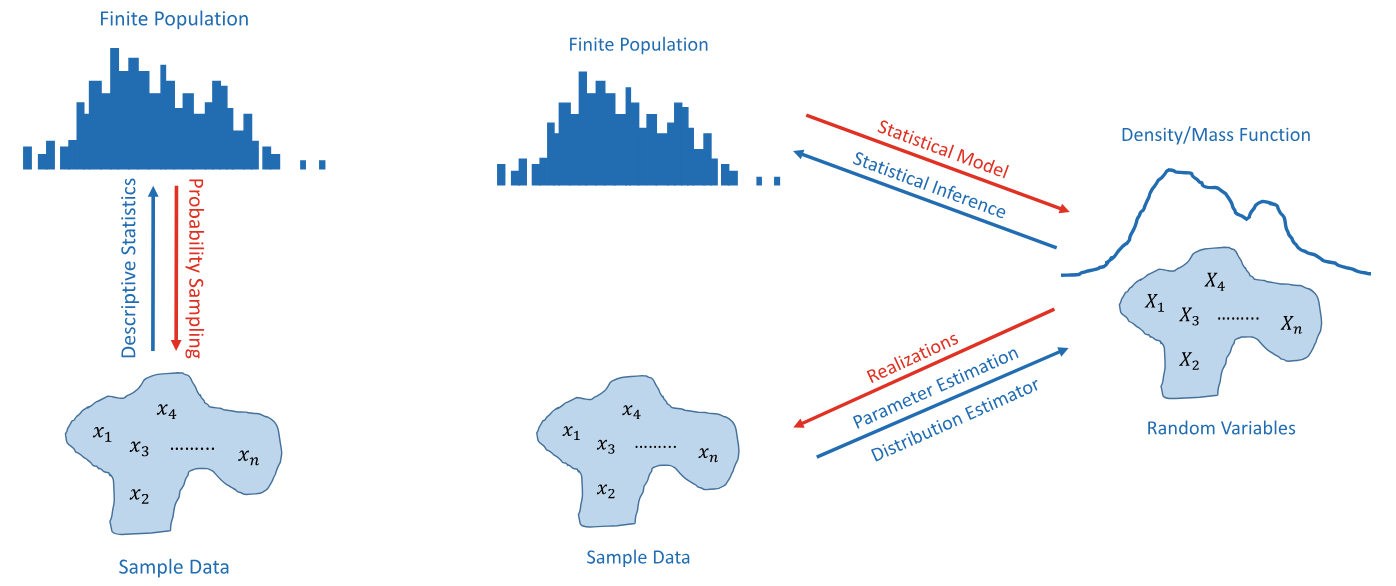
\includegraphics[
        width=\linewidth,
        height=5cm,
        keepaspectratio,
    ]{images/statistics/population-statistics-estimation.png}
    \caption*{
        we use the theory of random variables and distribution functions allows us to make more detailed statements about the population of interest
        \cite{statistics/book/Statistics-for-Data-Scientists/Maurits-Kaptein}
    }
\end{figure}


\begin{enumerate}
    \item Sample statistics are numerical values calculated from a sample (a subset of a population) to describe some aspect of the sample.
    \hfill \cite{common/online/chatgpt}

    \item An \textbf{estimator} is a rule or formula (usually a function of sample data) used to estimate a population parameter.
    \hfill \cite{common/online/chatgpt}

    \item These are statistics that summarize or describe features of a dataset.
    They can be from either a sample or an entire population.
    \hfill \cite{common/online/chatgpt}

    \item We are often interested in summarizing sets of random variables and comparing pairs of random variables.
    \hfill \cite{mfml/book/mml/Deisenroth-Faisal-Ong}

    \item A \textbf{statistic of a random variable} is a deterministic function of that random variable.
    \hfill \cite{mfml/book/mml/Deisenroth-Faisal-Ong}

    \item The summary statistics of a distribution provide one useful view of how a random variable behaves, and provides numbers that summarize and characterize the distribution.
    \hfill \cite{mfml/book/mml/Deisenroth-Faisal-Ong}

    \item Going from the data to the PDF or PMF to the population is also called statistical inference, but now we are using (parametric) statistical models.
    \hfill \cite{statistics/book/Statistics-for-Data-Scientists/Maurits-Kaptein}

    \item \textbf{Population Characterstics}:
    \begin{enumerate}
        \item \textbf{standardized variable};
        $
            Z = \dfrac{X - \mu( f )}{\sigma ( f )}
        $
        \hfill \cite{statistics/book/Statistics-for-Data-Scientists/Maurits-Kaptein}

        \item \textbf{population mean}:
        $
            \mu  ( f )
            = \mbbE[X]
            = \dint _\mbbR x f (x)dx
        $
        \hfill \cite{statistics/book/Statistics-for-Data-Scientists/Maurits-Kaptein}

        \item \textbf{population variance}:
        $
            \sigma ^2 ( f )
            = \mbbE [(X - \mu ( f ))^2]
            = \dint _\mbbR (x - \mu ( f ))^2 f (x) dx
        $
        \hfill \cite{statistics/book/Statistics-for-Data-Scientists/Maurits-Kaptein}

        \item \textbf{population standard deviation}:
        $
            \sigma ( f )
            = \sqrt{\sigma ^2 ( f ) }
        $
        \hfill \cite{statistics/book/Statistics-for-Data-Scientists/Maurits-Kaptein}

        \item \textbf{Third moment (skewness)}:
        $
            \gamma_1( f ) = \mbbE [(Z )^3]
        $
        \hfill \cite{statistics/book/Statistics-for-Data-Scientists/Maurits-Kaptein}

        \item \textbf{Fourth moment (excess kurtosis)}:
        $
            \gamma_2( f ) = \mbbE [(Z )^4]-3
        $
        \hfill \cite{statistics/book/Statistics-for-Data-Scientists/Maurits-Kaptein}

        \item \textbf{Quantiles}:
        $
            F (x _p ( f )) = \dint ^{x _p ( f )} _{-\infty} f (x) dx = p
            \Rightarrow
            x _p ( f ) = F^{-1} ( p)
        $
        \hfill \cite{statistics/book/Statistics-for-Data-Scientists/Maurits-Kaptein}
        \\
        $F^{-1}$ is the inverse distribution function
        \hfill \cite{statistics/book/Statistics-for-Data-Scientists/Maurits-Kaptein}

        \item [\textbf{Note}:] we are now using the notation $\mu ( f )$ to make explicit that the population mean $\mu$ will depend on our choice of $f$ .
        \hfill \cite{statistics/book/Statistics-for-Data-Scientists/Maurits-Kaptein}
    \end{enumerate}
\end{enumerate}





\subsection{Distributions of Sample Statistic $T_n$}


\begin{enumerate}
    \item \textbf{PMF or PDF}
    \hfill \cite{statistics/book/Statistics-for-Data-Scientists/Maurits-Kaptein}
    \begin{enumerate}
        \item In many settings, the sample distribution function has a sample PMF or PDF $f _{T_n}$ , often referred to as the sample density function of $T_n$ .
        \hfill \cite{statistics/book/Statistics-for-Data-Scientists/Maurits-Kaptein}

        \item  it is not always easy to determine the sample distribution or sample density function in general
        \hfill \cite{statistics/book/Statistics-for-Data-Scientists/Maurits-Kaptein}

        \item Only in special cases is it possible to determine closed-form functions.
        \hfill \cite{statistics/book/Statistics-for-Data-Scientists/Maurits-Kaptein}
    \end{enumerate}

    \item \textbf{CDF}: $F_{T_n} (x) = P (T_n \leq x)$
    \hfill \cite{statistics/book/Statistics-for-Data-Scientists/Maurits-Kaptein}
    \begin{enumerate}
        \item This CDF is often referred to as the sample distribution function of statistic $T_n$ , as it describes how the sample statistics vary if we draw (new) samples from the population.
        \hfill \cite{statistics/book/Statistics-for-Data-Scientists/Maurits-Kaptein}

    \end{enumerate}

    \item We study the distributions of $T_n$, as these distribution functions effectively allow us to examine the quality of our estimators: the distribution function of the random variable $T_n$ provides a measure of how well an estimator approximates a population value.
    \begin{enumerate}
        \item The expected value of an estimator $\mbbE[T_n]$ is a measure for the central tendency of a sample statistic
        \hfill \cite{statistics/book/Statistics-for-Data-Scientists/Maurits-Kaptein}

        \item The standard deviation of $T_n$ provides a measure for the variability of a sample statistic.
        The standard deviation of a sample statistic $T_n$ is the standard error of that sample statistic;
        the standard error of a sample statistic of interest is commonly reported in scientific texts to quantify the uncertainty associated with the sample statistic.
        \hfill \cite{statistics/book/Statistics-for-Data-Scientists/Maurits-Kaptein}
    \end{enumerate}
\end{enumerate}


\subsubsection{Distribution of the Sample Minimum}

\begin{enumerate}
    \item $F _{X_{(1)}}(x) = 1 - [1 - F(x)]^n$
    \hfill \cite{statistics/book/Statistics-for-Data-Scientists/Maurits-Kaptein}

    \item $f _{X_{(1)}} (x) = n [1 - F(x)]^{n-1}\ f (x)$
    \hfill \cite{statistics/book/Statistics-for-Data-Scientists/Maurits-Kaptein}
\end{enumerate}

\subsubsection{Distribution of the Sample Maximum}

\begin{enumerate}
    \item  Let $T_n$ be the maximum of $X_1 , X_2, \cdots , X _n$ , the distribution function of $T_n$ is given by:
    \hfill \cite{statistics/book/Statistics-for-Data-Scientists/Maurits-Kaptein}
    \\
    $
        \begin{aligned}
            F _{X_{(n)}} (x)
            &= P (X_{(n)} \leq x)
            = P (\max \dCurlyBrac{X_1, X_2, \cdots, X _n } \leq x) \\
            &= P (X_1 \leq x, X_2 \leq x, \cdots, X _n \leq x)
            = \dprod ^n _{i=1} P (X _i \leq x)
            = \dprod ^n _{i=1} F(x) \\
            &= [F (x)]^n
        \end{aligned}
        \hfill \text{\cite{statistics/book/Statistics-for-Data-Scientists/Maurits-Kaptein}}
    $

    \item $f _{X_{(n)}} (x) = n [F (x)]^{n-1}\ f (x)$
    \hfill \cite{statistics/book/Statistics-for-Data-Scientists/Maurits-Kaptein}
\end{enumerate}



\subsubsection{Distribution of the Sample Average}

\begin{enumerate}
    \item The distribution function of the sample average $\bar{X} = \dfrac{1}{n} \dsum^n _{i=1} X _i$ is not so easy to determine in general.
    \hfill \cite{statistics/book/Statistics-for-Data-Scientists/Maurits-Kaptein}

    \item The $p$-th moment of a general sample statistic $T_n$ is given by
    $\mbbE[T ^p _n] = \dint _\mbbR t^ p f _{T_n} (t) dt$,
    if the sample density $f _{T_n}$ exists, using the definition of moments for any random variable.
    \hfill \cite{statistics/book/Statistics-for-Data-Scientists/Maurits-Kaptein}

    \item  It can, however, also be calculated in a different way, using the population density $f$ and the fact that $X_1 , X_2, \cdots , X _n$ are i.i.d. $F$.
    The $p$-th moment of $T_n$ is:
    \hfill \cite{statistics/book/Statistics-for-Data-Scientists/Maurits-Kaptein}
    \\
    .\hfill
    $
        \begin{aligned}
            \mbbE[T ^p _n]
            &= \dint _\mbbR t ^p f_ {T_n} (t) dt
            = \mbbE[T ^p _n (X_1, X_2, \cdots , X _n )] \\
            &= \dint _{\mbbR^n} T ^p _n (x_1, x_2, \cdots , x _n )\ f (x_1) f (x_2) \cdots f (x _n ) \ dx_1dx_2 \cdots dx _n
        \end{aligned}
    $
    \hfill \cite{statistics/book/Statistics-for-Data-Scientists/Maurits-Kaptein}

    \item A special case is the first moment $\mu ( f_ {T_n} ) = \mbbE[T_n]$
    \hfill \cite{statistics/book/Statistics-for-Data-Scientists/Maurits-Kaptein}

    \item The advantage of $\mbbE[T ^p _n]$ equation is that the moments of the sample statistic $T_n = \bar{X}$ can be expressed in moments of the random variables $X_1 , X_2, \cdots , X _n$.
    Indeed, the first moment of $\bar{X}$ is now given by
    \hfill \cite{statistics/book/Statistics-for-Data-Scientists/Maurits-Kaptein}
    \\[0.3cm]
    .\hfill
    $
        \begin{aligned}
            \mu ( f _{\bar{X}} )
            &= \mbbE[\bar{X}]
            = \dint _{\mbbR^n} \dParenBrac{\dfrac{1}{n} \dsum ^n _{i=1} x_ i }\ f (x_1) f (x_2) \cdots f (x _n )\ dx_1dx_2 \cdots dx _n \\
            &= \dfrac{1}{n} \dsum^n _{i=1} \dint _{\mbbR^n} x _i\ f (x_1) f (x_2) \cdots f (x_ n )\ dx_1dx_2 \cdots dx _n
            = \dfrac{1}{n} \dsum^n _{i=1} \dint_ {\mbbR} x _i\ f (x _i )\ dx _i \\
            &= \dfrac{1}{n} \dsum^n _{i=1} \mbbE[X _i]
            = \mu ( f )
        \end{aligned}
        \hfill \text{\cite{statistics/book/Statistics-for-Data-Scientists/Maurits-Kaptein}}
    $

    \item The $p$-th central moment of $T_n$ is given by $\mbbE[(T_n - \mu( f _{T_n} ))^p] $
    \hfill \cite{statistics/book/Statistics-for-Data-Scientists/Maurits-Kaptein}
    \begin{enumerate}
        \item The second central moment is the variance of the sample statistic $T_n$.
        \hfill \cite{statistics/book/Statistics-for-Data-Scientists/Maurits-Kaptein}
        \\[0.2cm]
        .\hfill
        $
            \mbbE[( \bar{X} - \mu( f ))^2] = \dfrac{\sigma ^2( f )}{n}
        $
        \hfill \cite{statistics/book/Statistics-for-Data-Scientists/Maurits-Kaptein}

        \item Taking the square root second central moment, we obtain the standard deviation of $T_n$.
        \hfill \cite{statistics/book/Statistics-for-Data-Scientists/Maurits-Kaptein}
    \end{enumerate}

    \item The sample average has an expectation of $\mu ( f )$ and a variance of $\dfrac{\sigma  ^2 ( f )}{n}$, irrespective of the population density $f$ .
    In other words, the sample average $\bar{X}$ is an appropriate estimator for the population mean $\mu ( f )$, and it has a standard error (SE) that is a factor $\sqrt{n}$ smaller than the standard deviation of the population, i.e. the standard error is \colorbox{yellow}{$SE( \bar{X} ) = \dfrac{\sigma  ( f )}{\sqrt{n}}$}.
    Note that this standard error is typically unknown, since it depends on the unknown population standard deviation $\sigma ( f )$.
    This unknown parameter can also be estimated from the sample data.
    \hfill \cite{statistics/book/Statistics-for-Data-Scientists/Maurits-Kaptein}

    \item The skewness is given by \colorbox{yellow}{$\gamma _1( f _{\bar{X}} ) = \dfrac{\gamma _1( f )}{\sqrt{n}}$} and
    the excess kurtosis is given by \colorbox{yellow}{$\gamma _2( f _{\bar{X}} ) = \dfrac{\gamma _2( f )}{n}$}.
    Thus the skewness and excess kurtosis are close to zero when the sample size is getting large.
    \hfill \cite{statistics/book/Statistics-for-Data-Scientists/Maurits-Kaptein}
\end{enumerate}








\subsubsection{Distribution of the Sample Variance}

\begin{enumerate}
    \item The distribution function of the sample variance $T_n = S^2 \equiv \dfrac{1}{n - 1} \dsum ^n _{i=1}(X _i - \bar{X})^2$ is in general unknown, but we are able to determine a few moments.
    \hfill \cite{statistics/book/Statistics-for-Data-Scientists/Maurits-Kaptein}

    \item we can rewrite the variance first into
    $S^2 = \dfrac{1}{n - 1} \dParenBrac{\dsum^n _{i=1} (X _i - \mu ( f ))^2} - \dfrac{n( \bar{X} - \mu ( f ))^2}{n - 1}$
    \hfill \cite{statistics/book/Statistics-for-Data-Scientists/Maurits-Kaptein}

    \item first moment:
    \\[0.2cm]
    .\hfill
    $
        \begin{aligned}
            \mu  ( f _{S^2} )
            & = \mbbE[S^2] \\
            &= \dfrac{1}{n-1} \dsum^n _{i=1} \mbbE[(X _i - \mu ( f ))^2] - \dfrac{n}{n-1} \mbbE[( \bar{X} - \mu ( f ))^2] \\
            &= \dfrac{1}{n-1} (n\sigma ^ 2( f )) - \dfrac{n }{n-1} \dfrac{\sigma  ^2( f )}{n}
            = \dfrac{n}{n-1} \sigma ^ 2( f ) - \dfrac{1 }{n-1} \sigma  ^2( f )
            = \sigma ^2( f )
        \end{aligned}
        \hfill \text{\cite{statistics/book/Statistics-for-Data-Scientists/Maurits-Kaptein}}
    $

    \item The sample variance $S^2$ is an unbiased estimator of the population variance $\sigma ^2( f )$.
    \hfill \cite{statistics/book/Statistics-for-Data-Scientists/Maurits-Kaptein}

    \item estimate the standard error of the sample average: $\hat{SE}(\bar{X}) = \dfrac{S}{\sqrt{n}}$
    \hfill \cite{statistics/book/Statistics-for-Data-Scientists/Maurits-Kaptein}

    \item The second moment of the sample variance is more difficult to determine, but it is possible.
    \hfill \cite{statistics/book/Statistics-for-Data-Scientists/Maurits-Kaptein}
    \\[0.2cm]
    .\hfill
    $
        \sigma  ^2 ( f _{S^2} )
        = \mbbE[(S^2 - \mu ( f _{S^2} ))^2 ]
        = \mbbE[(S^2 - \sigma  ^2 ( f ))^2]
        = \dParenBrac{\dfrac{1}{n} \gamma_2 ( f ) + \dfrac{2}{n - 1}} \sigma  ^4 ( f )
    $
    \hfill \cite{statistics/book/Statistics-for-Data-Scientists/Maurits-Kaptein}

    \item The standard deviation
    \colorbox{yellow}{$\sigma ( f _{S^2} ) = \sigma ^2( f )\sqrt{\dfrac{(n - 1)\ \gamma_2( f ) + 2n}{n(n - 1)}}$}
    is also referred to as the standard error of the sample variance $S^2$.
    \hfill \cite{statistics/book/Statistics-for-Data-Scientists/Maurits-Kaptein}

    \item \textbf{standard error}:
    $\hat{SE}(S^2) = S^2\sqrt{\dfrac{(n - 1)\ b_2 + 2n}{n(n - 1)}}$
    \hfill \cite{statistics/book/Statistics-for-Data-Scientists/Maurits-Kaptein}
\end{enumerate}


\subsection{Central Limit Theorem (CLT)}

\begin{enumerate}
    \item  If the sample size increases, the standard deviation vanishes ($\dfrac{\sigma (f)}{\sqrt{n}} \to 0$ if $n \to \infty$).
    This implies that the sample average converges to the population mean $\mu( f )$.
    \hfill \cite{statistics/book/Statistics-for-Data-Scientists/Maurits-Kaptein}

    \item
    \begin{theorem}[Central Limit Theorem (CLT) (Lindeberg-Levy)]
        If we study the standardized sample average, i.e.
        $
            Z _n
            = \dfrac{\bar{X} - \mu ( f )}{\sigma  ( f )/\sqrt{n}}
            = \dfrac{\sqrt{n}( \bar{X} - \mu ( f ))}{\sigma  ( f )}
        $
        , the mean would be equal to zero ($\mbbE[Z _n] = 0$) and the variance would be equal to one ($\mbbE[Z ^2 _n] = 1$).
        This is true irrespective of the sample size $n$.
        \hfill \cite{statistics/book/Statistics-for-Data-Scientists/Maurits-Kaptein}
    \end{theorem}

    \item Note that the distribution function of $Z _n$ may still depend on $n$, since the skewness and kurtosis of $Z _n$ are given by $\dfrac{\gamma_1( f )}{\sqrt{n}}$ and $\dfrac{\gamma_2( f )}{n}$, respectively, and are different for different $n$.
    \hfill \cite{statistics/book/Statistics-for-Data-Scientists/Maurits-Kaptein}

    \item If the sample size becomes large, $Z _n = \dfrac{\sqrt{n}( \bar{X} - \mu ( f ))}{\sigma  ( f )} \sim \mathcal{N} (0, 1)$, becomes almost normal.
    \hfill \cite{statistics/book/Statistics-for-Data-Scientists/Maurits-Kaptein}

    \item Note that it did not imply anything about the shape of the population density $f$ , just the existence of $\mu( f )$ and $\sigma^ 2( f )$ (and of course the assumption that $X_1 , X_2, \cdots , X _n$ are i.i.d. with density $f$ ).
    \hfill \cite{statistics/book/Statistics-for-Data-Scientists/Maurits-Kaptein}

    \item Any statistic of the form $S_n = \dfrac{1}{n} \dsum^n _{i=1} \psi(X _i )$ would also converge to a normal distribution function when the mean $\mu_\psi ( f ) = \mbbE[\psi(X _k])$ and variance $\sigma ^2 _\psi  ( f ) = \mbbE[(\psi (X _k ) - \mu_\psi  ( f ))^2]$ are finite.
    \hfill \cite{statistics/book/Statistics-for-Data-Scientists/Maurits-Kaptein}

    \item Using the central limit theorem, $\psi (X_1), \psi (X_2), \cdots , \psi (X_ n )$ are i.i.d. and have a finite variance; thus, the statistic $\sqrt{n}(S_n - \mu_\psi  ( f ))$ converges to a normal distribution with mean zero and variance $\sigma^ 2 _\psi  ( f )$.
    \hfill \cite{statistics/book/Statistics-for-Data-Scientists/Maurits-Kaptein}
\end{enumerate}



\subsubsection{Central Limit Theorem Applied to Variances}

\begin{enumerate}
    \item The central limit theorem can also be applied to the sample variance $S^2$ , when the fourth central moment $\mbbE[(X _k - \mu( f ))^4]$ exists.
    The sample variance can be rewritten as
    \hfill \cite{statistics/book/Statistics-for-Data-Scientists/Maurits-Kaptein}
    \\
    .\hfill
    $
        S^2 = \dfrac{1}{n - 1} \dsum^n _{i=1} (X _i - \mu( f ))^2 - \dfrac{n}{n - 1} (\bar{X} - \mu( f ))^2
    $
    \hfill \cite{statistics/book/Statistics-for-Data-Scientists/Maurits-Kaptein}

    \item We may apply the central limit theorem to $\dfrac{1}{ n} \dsum ^n _{i=1} (X_ i - \mu  ( f ))^2$ , where $\psi(x) = (x - \mu ( f ))^2$ .
    \hfill \cite{statistics/book/Statistics-for-Data-Scientists/Maurits-Kaptein}
    \begin{enumerate}
        \item \textbf{mean}: $\mu _\psi ( f ) = \mbbE[(X _i - \mu ( f ))^2] = \sigma ^2( f )$
        \hfill \cite{statistics/book/Statistics-for-Data-Scientists/Maurits-Kaptein}

        \item \textbf{variance}:
        $
            \begin{aligned}
                \sigma  ^2 _\psi ( f )
                &= \mbbE[((X _i - \mu ( f ))^2 - \sigma ^ 2( f ))^2 ] \\
                &= \mbbE[(X _i - \mu ( f ))^4] - \sigma ^ 4( f )
                = (\gamma_2( f ) + 2)\ \sigma  ^4( f )
            \end{aligned}
        $
        \hfill \cite{statistics/book/Statistics-for-Data-Scientists/Maurits-Kaptein}

        \item
        $
            \mbbV\dSquareBrac{\dfrac{1}{n} \dsum^n _{i=1}(X _i - \mu ( f ))^2}
            = \dfrac{(\gamma_2( f ) + 2)\ \sigma^ 4( f )}{n}
        $
        \hfill \cite{statistics/book/Statistics-for-Data-Scientists/Maurits-Kaptein}
        \begin{enumerate}
            \item
            $
                \dfrac{1}{\sqrt{n}} \dsum^n _{i=1} [(X _i - \mu ( f ))^2 - \sigma ^2( f )]
                \overset{n \to \infty}{\longrightarrow}
                \mathcal{N}\dParenBrac{0,  [\gamma_2( f ) + 2]\sigma ^4( f )}
            $
            \hfill \cite{statistics/book/Statistics-for-Data-Scientists/Maurits-Kaptein}

            \item $\dfrac{1}{ n} \dsum^n _{i=1}(X _i - \mu ( f ))^2$ is approximately normally distributed with $\mathcal{N} \dParenBrac{\sigma ^ 2( f ), \dfrac{[\gamma_2( f ) + 2]\ \sigma  ^4 ( f )}{N}}$,
            which implies that $\dfrac{1}{n-1} \dsum^n _{i=1}(X_ i - \mu ( f ))^2$ is approximately normally distributed with
            \\[0.2cm]
            $\mathcal{N} \dParenBrac{\sigma ^ 2( f ), \dfrac{[\gamma_2( f ) + 2]\ \sigma ^ 4( f )}{n}}$.
            \hfill \cite{statistics/book/Statistics-for-Data-Scientists/Maurits-Kaptein}
        \end{enumerate}
    \end{enumerate}

    \item The distribution of $\sqrt{n}( \bar{X} - \mu( f ))$ converges to the normal distribution $\mathcal{N} (0, \sigma ^2( f ))$.
    \hfill \cite{statistics/book/Statistics-for-Data-Scientists/Maurits-Kaptein}
    \begin{enumerate}
        \item
        $
            ( \bar{X} - \mu ( f ))^2
            = \dfrac{[\sqrt{n}( \bar{X} - \mu ( f ))]^2}{n} \to 0
        $
        when $n$ converges to $\infty$
        \hfill \cite{statistics/book/Statistics-for-Data-Scientists/Maurits-Kaptein}
    \end{enumerate}

    \item $\sqrt{n}(S^2 - \sigma  ^2( f ))$ converges to a normal distribution  $\mathcal{N} (0, [\gamma_2( f ) + 2]\ \sigma ^ 4( f ))$, with $\sigma ^ 2( f )$ the population variance and $\gamma_2( f )$ the population excess kurtosis.
    \hfill \cite{statistics/book/Statistics-for-Data-Scientists/Maurits-Kaptein}
\end{enumerate}








\subsection{Asymptotic Confidence Intervals}

\begin{enumerate}
    \item The sample distribution function $F_{T_n}$ can help quantify how much the statistic is varying around the population characteristic it is trying to approach.
    \hfill \cite{statistics/book/Statistics-for-Data-Scientists/Maurits-Kaptein}

    \item Based on the definition of quantiles and the sampling distribution function $F_{T_n}$ , the sample statistic will fall in the interval $(x _p ( f _{T_n} ),\ x_{1- p} ( f _{T_n} )]$ with probability $1 - 2 p$.
    \hfill \cite{statistics/book/Statistics-for-Data-Scientists/Maurits-Kaptein}

    \item
    $
        \begin{aligned}
            P(T_n \in (x_ p ( f _{T_n} ),\ x_{1- p} ( f _{T_n} )])
            &= P(T_n \leq  x_{1- p} ( f _{T_n} )) - P(T_n \leq  x_ p ( f _{T_n} )) \\
            &= F_{T_n} (x_{1- p} ( f _{T_n} )) - F_{T_n} (x _p ( f _{T_n} )) \\
            &= 1 - p - p = 1 - 2 p
        \end{aligned}
        \hfill \text{\cite{statistics/book/Statistics-for-Data-Scientists/Maurits-Kaptein}}
    $

    \item If $\tau_n$ is \textbf{the standard error} of the sample statistic $T_n$, $z _p = x _p (\phi)$ is the quantile of the standard normal distribution, then the sample statistic $T_n$ falls in the interval $(\theta  + z _p \tau_ n ,\ \theta  + z_{1- p} \tau _n ] = (\theta  - z_{1- p} \tau _n , \theta  + z_{1- p} \tau_ n ]$ with probability approximately equal to $1 - 2 p$.
    \hfill \cite{statistics/book/Statistics-for-Data-Scientists/Maurits-Kaptein}

    \item
    $
        \begin{aligned}
            &P(T_n \in  (\theta  - z_{1- p} \tau_n ,\ \theta  + z_{1- p} \tau_n ]) \\
            &= P((T_n - \theta )/\tau_n \in  (-z{1- p} ,\ z{1- p} ]) \\
            &\approx \Phi(z_{1- p} ) - \Phi(-z_{1- p} ) \\
            &= 1 - p - p
            = 1 - 2 p
        \end{aligned}
        \hfill \text{\cite{statistics/book/Statistics-for-Data-Scientists/Maurits-Kaptein}}
    $

    \item We can rewrite the probability $P(T_n \in  (\theta  - z_{1- p} \tau _n ,\ \theta  + z_{1- p} \tau_ n ])$ into $P(\theta  \in  (T_n - z_{1- p} \tau _n ,\ T_n + z_{1- p} \tau _n ])$, which means that the population characteristic is contained within limits $T_n - z_{1- p} \tau _n$ and $T_n + z_{1- p} \tau _n$ with probability equal to $1 - 2 p$.
    \hfill \cite{statistics/book/Statistics-for-Data-Scientists/Maurits-Kaptein}

    \item The interval $(T_n - z_{1- p} \tau_n , T_n + z_{1- p} \tau_n ]$ is now called an \textbf{asymptotic confidence interval} for $\theta$ with confidence level $1 - 2 p$.
    \hfill \cite{statistics/book/Statistics-for-Data-Scientists/Maurits-Kaptein}

    \item In practice we still need to estimate the standard error $\tau_n$ to be able to calculate the confidence interval, as $\tau_n$ would be a function of the density parameters and is unknown in the calculation of the interval $(T_n - z_{1- p} \tau_n , T_n + z_{1- p} \tau_n ]$.
    \hfill \cite{statistics/book/Statistics-for-Data-Scientists/Maurits-Kaptein}
    \begin{enumerate}
        \item It is then common to replace $\tau_n$ by its estimator $\hat{\tau}_n$ .
        \hfill \cite{statistics/book/Statistics-for-Data-Scientists/Maurits-Kaptein}

        \item In some cases, we would also change the normal quantile $z_{1- p}$ by a quantile of the $t$-distribution if we could formulate a degrees of freedom for the estimator $\hat{\tau}_n$
        \hfill \cite{statistics/book/Statistics-for-Data-Scientists/Maurits-Kaptein}
    \end{enumerate}
\end{enumerate}


\subsection{Methods of Estimation: Method of Moments Estimation (MME)}

\begin{enumerate}
    \item Assume that the population density $f_{\bm{\theta} }$ depends on a set of parameters $\bm{\theta}  = (\theta _1, \theta _2, \cdots , \theta _m )^\top$
    \hfill \cite{statistics/book/Statistics-for-Data-Scientists/Maurits-Kaptein}

    \item Estimates of these parameters can then be obtained by computing $m$ or more central moments.
    \hfill \cite{statistics/book/Statistics-for-Data-Scientists/Maurits-Kaptein}

    \item
    $
        \mu_r ( f_{\bm{\theta}} )
        = \mbbE [(X - \mu ( f_{\bm{\theta}} ))^r ]
        =
        \begin{cases}
            \dint _{\mbbR} (x - \mu ( f_{\bm{\theta}} ))^r\ f_{\bm{\theta}} (x)\ dx & \text{ continuous} \\
            \dsum _{k=0}^{\bm{\theta}} (k - \mu ( f_{\bm{\theta}} ))^r\ f_{\bm{\theta}} (k) & \text{ discrete} \\
        \end{cases}
    $
    where
    \hfill \cite{statistics/book/Statistics-for-Data-Scientists/Maurits-Kaptein}
    \begin{enumerate}
        \item  $\mu( f_{\bm{\theta}} ) = \mbbE[X]$ the mean value
        \hfill \cite{statistics/book/Statistics-for-Data-Scientists/Maurits-Kaptein}

        \item $f_{\bm{\theta}} (k)$ represents the probability that $X$ is equal to $k$
        \hfill \cite{statistics/book/Statistics-for-Data-Scientists/Maurits-Kaptein}
    \end{enumerate}

    \item The moments can be estimated with the sample moments $M_r = \dfrac{1}{n} \dsum^n _{i=1} (X_ i - \bar{X} )^r$ with $M_1 = \bar{X}$ and $\bar{X}$ the sample average.
    \hfill \cite{statistics/book/Statistics-for-Data-Scientists/Maurits-Kaptein}

    \item If we equate the sample moments $M_r$ to the centralized population moments $\mu_r$ , we create a system of equations that can possible be solved for $\bm{\theta}$.
    \hfill \cite{statistics/book/Statistics-for-Data-Scientists/Maurits-Kaptein}

    \item When executing the method of moments, we are looking for parameters $\bm{\theta } = (\theta _1, \theta _2, \cdots , \theta _m )^\top$ that satisfy the following equations $\bar{X} = \mu ( f_{\bm{\theta}}  )$ and $M_r = \mu_r ( f_{\bm{\theta}}  )$ for $r = 2, 3, \cdots , m$.
    \hfill \cite{statistics/book/Statistics-for-Data-Scientists/Maurits-Kaptein}

    \item The solution $\tilde{\bm{\theta}} = ( \tilde{\theta}_1, \tilde{\theta}_2, \cdots , \tilde{\theta}_m )^\top$ is called the \textbf{method of moments estimator}.
    \hfill \cite{statistics/book/Statistics-for-Data-Scientists/Maurits-Kaptein}

    \item Note that the second sample moment ($M_2$) is equal to $\dfrac{(n - 1)}{n}S^2$ and is thus not an unbiased estimator of $\mu_r ( f_{\bm{\theta}} )$, since we already now that $S^2$ is unbiased.
    \hfill \cite{statistics/book/Statistics-for-Data-Scientists/Maurits-Kaptein}

    \item The moment estimators on transformed data are different from the moment estimators on the original data
    \hfill \cite{statistics/book/Statistics-for-Data-Scientists/Maurits-Kaptein}

    \item The non-uniqueness issue is considered a real disadvantage of the moment estimators.
    \hfill \cite{statistics/book/Statistics-for-Data-Scientists/Maurits-Kaptein}
\end{enumerate}




\subsection{Methods of Estimation: Maximum Likelihood Estimation (MLE)}

\begin{enumerate}
    \item If $X_1 , X_2, \cdots , X_n$ are i.i.d. with density $f_{\bm{\theta}}$ , the likelihood function is given by $L (\bm{\theta}|X_1, X_2, \cdots , X_n ) = \dprod^n _{i=1} f_{\bm{\theta}} (X_i )$ and the log likelihood function is given by
    % \hfill \cite{statistics/book/Statistics-for-Data-Scientists/Maurits-Kaptein}
    % \\
    % .\hfill
    $
        \ell_{\bm{\theta}}
        \equiv (\bm{\theta}|X_1, X_2, \cdots , X_n )
        = \dsum ^n _{i=1} \log f_{\bm{\theta}} (X_i )
    $
    \hfill \cite{statistics/book/Statistics-for-Data-Scientists/Maurits-Kaptein}

    \item The maximum likelihood estimator $\hat{\bm{\theta}} = ( \hat{\theta}_1, \hat{\theta}_2, \cdots , \hat{\theta}_n )^\top$ is the set of parameters that maximizes the log likelihood function.
    It is considered a (vector of) random variable(s), since it is a (set of) function(s) of the random variables $X_1 , X_2, \cdots , X _n $.
    \hfill \cite{statistics/book/Statistics-for-Data-Scientists/Maurits-Kaptein}

    \item $X_1 , X_2, \cdots , X _n $ can often be determined by solving the set of equations given by
    \hfill \cite{statistics/book/Statistics-for-Data-Scientists/Maurits-Kaptein}
    \\[0.2cm]
    .\hfill
    $
        \dfrac{\partial \ell_{\bm{\theta}}}{\partial\theta_k}
        = \dsum^n _{i=1} \dParenBrac{
            \dfrac{1}{f_{\bm{\theta}} (X _i )}
            \dfrac{\partial f_{\bm{\theta}} (X_i )}{\partial\theta_k}
        }
        = 0
    $
    \hfill \cite{statistics/book/Statistics-for-Data-Scientists/Maurits-Kaptein}
    \\[0.2cm]
    This set of equations is often referred to as the \textbf{likelihood equations}.
    \hfill \cite{statistics/book/Statistics-for-Data-Scientists/Maurits-Kaptein}

    \item The solution $\hat{\bm{\theta}}$ does not always result in a closed form expression, which means that we have to resort to numerical approaches if we want to determine the MLE on data.
    \hfill \cite{statistics/book/Statistics-for-Data-Scientists/Maurits-Kaptein}

    \item This is often considered a drawback of the MLE.
    It may estimate the parameters of the PDF or PMF unbiasedly, but they do not always estimate the population mean and variance unbiasedly.
    This would be different from the moment estimators applied to the original scale of the observations.
    \hfill \cite{statistics/book/Statistics-for-Data-Scientists/Maurits-Kaptein}
\end{enumerate}



\subsubsection{Standard Error of MLE}

\begin{enumerate}
    \item The standard errors of the maximum likelihood estimators are calculated based on the variance of the large sample distribution (or asymptotics) of the maximum likelihood estimators.
    \hfill \cite{statistics/book/Statistics-for-Data-Scientists/Maurits-Kaptein}

    \item Under certain regularity conditions, it can be shown that $\sqrt{n}(\hat{\bm{\theta}} - \bm{\theta})$ converges to a normal distribution $\mathcal{N} (0, I ^{-1} (\bm{\theta}))$, with $\hat{\bm{\theta}}$ the MLE and $I (\bm{\theta})$ the so-called Fisher information.
    \hfill \cite{statistics/book/Statistics-for-Data-Scientists/Maurits-Kaptein}
\end{enumerate}


\vspace{0.5cm}
\textbf{(Informal) Illustrative proof}:
\begin{enumerate}
    \item we will assume that the density $f_{\theta}$ has only one parameter instead of multiple parameters $\theta_1 , \theta_2, \cdots , \theta_m $.
    \hfill \cite{statistics/book/Statistics-for-Data-Scientists/Maurits-Kaptein}

    \item The first derivative of the log likelihood, which is also referred to as the score function $S(\theta)$, is given by
    % \hfill \cite{statistics/book/Statistics-for-Data-Scientists/Maurits-Kaptein}
    % \\
    % .\hfill
    $
        S_n (\theta )
        \equiv \dfrac{d\ell\theta }{d\theta}
        = \dsum^n _{i=1} \dfrac{d} {d\theta}  \log f_\theta  (X_i )
        = \dsum^n _{i=1} \dfrac{f^\prime_\theta  (X_i ) }{f_{\theta}  (X_i )}
    $
    \hfill \cite{statistics/book/Statistics-for-Data-Scientists/Maurits-Kaptein}

    \item The expectation of the score function is zero (under certain regularity conditions), since
    \hfill \cite{statistics/book/Statistics-for-Data-Scientists/Maurits-Kaptein}
    \\[0.2cm]
    .\hfill
    $
        \mbbE\dSquareBrac{\dfrac{f ^\prime _\theta  (X_i )}{f_\theta  (X_i )}}
        = \dint _\mbbR f ^\prime _\theta  (x)dx
        = \dfrac{d} {d\theta}  \dint _\mbbR f_\theta  (x)dx
        = 0
    $
    \hfill \cite{statistics/book/Statistics-for-Data-Scientists/Maurits-Kaptein}
    \\[0.2cm]
    This implies that $\mbbE[S_n (\theta)] = 0$.
    \hfill \cite{statistics/book/Statistics-for-Data-Scientists/Maurits-Kaptein}

    \item The variance of the score function is now given by $\mbbE[S^2 _n (\theta )] = n \dint _\mbbR\dfrac{( f ^\prime _\theta  (x))^2}{f_\theta  (x)}dx$.
    \hfill \cite{statistics/book/Statistics-for-Data-Scientists/Maurits-Kaptein}

    \item \textbf{Fisher information}:
    % \hfill \cite{statistics/book/Statistics-for-Data-Scientists/Maurits-Kaptein}
    % \\
    % .\hfill
    $
        I (\theta )
        = \mbbE \dSquareBrac{\dParenBrac{\dfrac{d \log f_\theta  (X)}{d\theta }}^2 }
        = \dint _\mbbR \dfrac{( f ^\prime _\theta  (x))^2}{ f_\theta  (x)} dx
    $
    \hfill \cite{statistics/book/Statistics-for-Data-Scientists/Maurits-Kaptein}

    \item The score function is a sum of independent random variables, which means that if we standardize the score function appropriately, the central limit theorem tells us that the distribution function of the score function will converge to a normal distribution function.
    $S_n (\theta)/\sqrt{n\ I (\theta)}$ converges to a standard normal random variable $Z \sim \mathcal{N} (0, 1)$.
    \hfill \cite{statistics/book/Statistics-for-Data-Scientists/Maurits-Kaptein}

    \item The Fisher information is equal to the minus expectation of the derivative of the score function with respect to the parameter $\theta$, i.e. $n\ I (\theta) = -\mbbE[S^\prime_n (\theta)]$ with $S^\prime_n (\theta) = \dfrac{dS_n (\theta)}{d\theta}$.
    \hfill \cite{statistics/book/Statistics-for-Data-Scientists/Maurits-Kaptein}

    \item $S^\prime_n (\theta)$ is also a sum of independent random variables; thus properly standardized it will converge to a standard normal random variable.
    This also implies that $\dfrac{S^\prime _n (\theta)}{n}$ will converge to the Fisher information $I (\theta)$ .
    \hfill \cite{statistics/book/Statistics-for-Data-Scientists/Maurits-Kaptein}

    \item using a first-order Taylor expansion for the score function $S_n ( \hat{\theta})$ that is evaluated in the ML estimator $\hat{\theta}$, we obtain that $S_n ( \hat{\theta}) \approx S_n (\theta) + ( \hat{\theta} - \theta)\ S^\prime_n (\theta)$.
    But the score function in the MLE estimator is zero, i.e. $S_n ( \hat{\theta}) = 0$, since the MLE estimator $\hat{\theta}$ maximizes the likelihood. This means that
    \hfill \cite{statistics/book/Statistics-for-Data-Scientists/Maurits-Kaptein}
    \\[0.2cm]
    .\hfill
    $
        \sqrt{n}( \hat{\theta} - \theta)
        \approx - \dfrac{\sqrt{n}S_n (\theta)}{ S^\prime_n (\theta) }
        = - \dfrac{1 }{\sqrt{I (\theta)}} \dfrac{S_n (\theta)}{\sqrt{n I (\theta)}} \dfrac{n I (\theta)}{S^\prime_n (\theta)}
    $
    \hfill \cite{statistics/book/Statistics-for-Data-Scientists/Maurits-Kaptein}

    \item Since $\dfrac{n I (\theta)}{S^\prime _n (\theta)}$ converges to $1$ and $\dfrac{S_n (\theta)}{\sqrt{n I (\theta)}}$ converges to $Z \sim \mathcal{N} (0, 1)$, we obtain that $\sqrt{n}( \hat{\theta} - \theta)$ converges to $\mathcal{N} \dParenBrac{0,\ \dfrac{1}{I (\theta)}}$.
    \hfill \cite{statistics/book/Statistics-for-Data-Scientists/Maurits-Kaptein}

    \item we see that the asymptotic variance of the maximum likelihood estimator is $I ^{-1}(\theta)$.
    \hfill \cite{statistics/book/Statistics-for-Data-Scientists/Maurits-Kaptein}

    \item This implies that the approximate standard error (or asymptotic standard error) of the maximum likelihood estimator is now $S E( \hat{\theta}) = \dfrac{1}{\sqrt{n I (\theta)}}$.
    Since we have an estimator $\hat{\theta}$ of the parameter $\theta$, the standard error is estimated with $\hat{SE}( \hat{\theta}) = \dfrac{1}{\sqrt{n I (\hat{\theta})}}$.
    This asymptotic standard error ($S E( \hat{\theta})$) can be used in the calculation of confidence intervals on $\theta$.
    \hfill \cite{statistics/book/Statistics-for-Data-Scientists/Maurits-Kaptein}

    \item When $T_n = \hat{\theta}$ is the MLE for $\theta$ having an estimated standard error $\hat{\tau}_n = \dfrac{1}{\sqrt{n I ( \hat{\theta})}}$, the $1 - 2 p$ asymptotic confidence interval is
    $
        \left(
        \dfrac{\hat{\theta} - z_{1-p}} {\sqrt{n I ( \hat{\theta})}},
        \ \dfrac{\hat{\theta} + z_{1-p}} {\sqrt{n I ( \hat{\theta})} }
        \right]
    $
    \hfill \cite{statistics/book/Statistics-for-Data-Scientists/Maurits-Kaptein}
\end{enumerate}






\section{Expected Values ($E(X)$)}

\begin{enumerate}
    \item \textbf{Covariance}: Covariance measures how two variables change together. If one variable increases when the other increases, the covariance is positive; if one decreases when the other increases, it's negative.
    \hfill \cite{common/online/chatgpt}
    \begin{enumerate}
        \item Units depend on the original variables.
        \hfill \cite{common/online/chatgpt}

        \item Hard to interpret the strength of the relationship due to unit dependence.
        \hfill \cite{common/online/chatgpt}

        \item Sensitive to scale.
        \hfill \cite{common/online/chatgpt}
    \end{enumerate}

    \item \textbf{Correlation}: Correlation standardizes covariance and measures both direction and strength of a linear relationship between two variables.
    \hfill \cite{common/online/chatgpt}
    \begin{enumerate}
        \item Always between $-1$ and $+1$.
        \hfill \cite{common/online/chatgpt}

        \begin{enumerate}
            \item $+1$: perfect positive linear relationship
            \hfill \cite{common/online/chatgpt}

            \item $0$: no linear relationship
            \hfill \cite{common/online/chatgpt}

            \item $-1$: perfect negative linear relationship
            \hfill \cite{common/online/chatgpt}
        \end{enumerate}

        \item Unitless.
        \hfill \cite{common/online/chatgpt}

        \item Easier to interpret than covariance.
        \hfill \cite{common/online/chatgpt}
    \end{enumerate}

    \item \textbf{Causation}: Causation means that changes in one variable directly cause changes in another.
    \hfill \cite{common/online/chatgpt}
    \begin{enumerate}
        \item Implies a cause-and-effect relationship.
        \hfill \cite{common/online/chatgpt}

        \item Cannot be determined just by looking at data or statistical relationships.
        \hfill \cite{common/online/chatgpt}

        \item Requires controlled experiments or strong observational evidence (e.g., through randomized trials or causal inference techniques).
        \hfill \cite{common/online/chatgpt}
    \end{enumerate}
\end{enumerate}




\subsection{For PDF (Continuous)}

\begin{enumerate}
    \item If we consider a (not necessarily continuous or differentiable) function $\psi : \mbbR \to \mbbR$, then the expected value of the random variable $\psi (X)$ is defined by
    \colorbox{yellow}{$
        \mbbE[\psi(X)]
        = \dint_{\mbbR} \psi(x)\ f(x)\ dx
    $}
    \hfill \cite{statistics/book/Statistics-for-Data-Scientists/Maurits-Kaptein}
\end{enumerate}




\subsection{For PMF (Discrete)}

\begin{enumerate}
    \item The expectation of a discrete random variable $\psi(X)$ is given by
    \hfill \cite{statistics/book/Statistics-for-Data-Scientists/Maurits-Kaptein}
    \\[0.2cm]
    \colorbox{yellow}{$
        \mbbE[\psi(X)] \
        = \dsum^{\infty}_{k=0}\ \psi(k)\ p _k \
        = \dsum^{\infty}_{k=0}\ \psi(k)\ P(X = k)
    $}
    \hfill \cite{statistics/book/Statistics-for-Data-Scientists/Maurits-Kaptein}

    \item If we would collect many realizations of the discrete random variable $X$, say $N$ realizations, we expect to see value $k$ with frequency $N \cdot p _k$ .
    \hfill \cite{statistics/book/Statistics-for-Data-Scientists/Maurits-Kaptein}
\end{enumerate}




\subsection{Common for PDF \& PMF}

\begin{enumerate}
    \item \textbf{First moment}: mean $\mu$ is obtained by \colorbox{yellow}{$\psi(x)=x$}
    \hfill \cite{statistics/book/Statistics-for-Data-Scientists/Maurits-Kaptein}

    \item \textbf{Second central moment}: The population variance $\sigma^ 2$ is obtained by \colorbox{yellow}{$\psi(x)=(x -\mu)^2$}
    \hfill \cite{statistics/book/Statistics-for-Data-Scientists/Maurits-Kaptein}

    \item \textbf{pth moment} of random variable $X$ is obtained by \colorbox{yellow}{$\psi(x) = x^p$}
    \hfill \cite{statistics/book/Statistics-for-Data-Scientists/Maurits-Kaptein}

    \item \textbf{pth central moment} of random variable $X$ is obtained by choosing \colorbox{yellow}{$\psi(x) = (x - \mu)^p$}
    \hfill \cite{statistics/book/Statistics-for-Data-Scientists/Maurits-Kaptein}

    \item \textbf{skewness}: \colorbox{yellow}{$\gamma_1 = \dfrac{\mu_3}{\sigma^3}$}, where $\mu_3 = \mbbE[(x-\mu)^3]$
    \hfill \cite{statistics/book/Statistics-for-Data-Scientists/Maurits-Kaptein}

    \item \textbf{kurtosis}: \colorbox{yellow}{$\gamma_2 = \dfrac{\mu_4}{\sigma^4} - 3$}, where $\mu_4 = \mbbE[(x-\mu)^4]$
    \hfill \cite{statistics/book/Statistics-for-Data-Scientists/Maurits-Kaptein}
\end{enumerate}

\vspace{0.5cm}
\textbf{Note}:
\begin{enumerate}
    \item the moments of a discrete random variable $X$ may \textbf{not} always exist: this depends on the choice of probabilities $p _k $.
    \hfill \cite{statistics/book/Statistics-for-Data-Scientists/Maurits-Kaptein}
\end{enumerate}











\section{Calculation Rules for Random Variables}

\begin{enumerate}
    \item Let we have 2 random variables $X, \ Y$, either discrete or continuous, and a constant $c$.

    \item $F _X$ and $F_Y$ the CDFs for $X$ and $Y$ , respectively. $P(X \leq x, Y \leq y)$ is the joint CDF of $X$ and $Y$ , denoted by $F _{X Y} (x, y)$

    \item Let events $A = \dCurlyBrac{X \leq x}$ and $B = \dCurlyBrac{Y \leq y}$

    \item the covariance is affected by transformations
\end{enumerate}


\subsection{Univariate/ Joint PMF/ PDF/ CDF}

\begin{enumerate}[series=calcrulesrv]
    \item The expected value of a function $g : \mbbR \to \mbbR$ of a univariate continuous random variable $X \sim P(x)$ is given by 
    \colorbox{yellow}{$\mbbE_X [g(x)] = \dint_ {\mathcal{X}} g(x)\ p(x)\ dx$}
    where $\mathcal{X}$ is the set of possible outcomes (the target space) of the random variable $X$.
    \hfill \cite{mfml/book/mml/Deisenroth-Faisal-Ong}
    \\[0.2cm]
    The expected value of a function of a random variable is sometimes referred to as the \textbf{law of the unconscious statistician}. 
    \hfill \cite{mfml/book/mml/Deisenroth-Faisal-Ong}
    \\
    It defines the meaning of the notation $\mbbE_X$ as the operator indicating that we should take the integral with respect to the probability density (for continuous distributions) or the sum over all states (for discrete distributions).
    \hfill \cite{mfml/book/mml/Deisenroth-Faisal-Ong}
    \\
    When the random variable associated with the expectation or covariance is clear by its arguments, the subscript is often suppressed (for example, $\mbbE_X [x]$ is often written as $\mbbE[x]$).
    \hfill \cite{mfml/book/mml/Deisenroth-Faisal-Ong}

    \item For multivariate random variables, we define the expected value element wise
    \hfill \cite{mfml/book/mml/Deisenroth-Faisal-Ong}
    \\[0.2cm]
    .\hfill
    $
        \mbbE_X [g(\bm{x})] = \begin{bmatrix}
            \mbbE_{X_1} [g(x_1)] \\ \vdots \\ \mbbE_{X_D} [g(x_D )]
        \end{bmatrix}
        \in \mbbR^D
    $
    \hfill \cite{mfml/book/mml/Deisenroth-Faisal-Ong}
    \\[0.2cm]
    where the subscript $\mbbE_{X_d}$ indicates that we are taking the expected value with respect to the $d$-th element of the vector $\bm{x}$.
    \hfill \cite{mfml/book/mml/Deisenroth-Faisal-Ong}

    \item The mean of a random variable $X$ with states $\bm{x} \in \mbbR^D$ is an average and is defined as
    \hfill \cite{mfml/book/mml/Deisenroth-Faisal-Ong}
    \\[0.2cm]
    .\hfill
    $
        \mbbE_X [\bm{x}] =
        \begin{bmatrix}
            \mbbE_{X_1} [x_1] \\
            \vdots \\
            \mbbE_{X_D} [x_D ]
        \end{bmatrix}
        \in \mbbR^D 
    $
    \hfill \cite{mfml/book/mml/Deisenroth-Faisal-Ong}
    \\[0.2cm]
    where
    \hfill \cite{mfml/book/mml/Deisenroth-Faisal-Ong}
    \\[0.2cm]
    .\hfill
    $
        \mbbE_{X_d} [x_d] :=
        \begin{cases}
            \dint_{\mathcal{X}} x_d\ p(x_d)\ dx_d & \text{ if $X$ is a continuous random variable} \\[0.2cm]
            \dsum_{x_i \in \mathcal{X}} x_i\ p(x_d = x_i) & \text{ if $X$ is a discrete random variable}
        \end{cases}
    $
    \hfill \cite{mfml/book/mml/Deisenroth-Faisal-Ong}
    \\[0.2cm]
    for $d = 1, \cdots , D$, where the subscript $d$ indicates the corresponding dimension of $\bm{x}$. 
    The integral and sum are over the states $\mathcal{X}$ of the target space of the random variable $X$.
    \hfill \cite{mfml/book/mml/Deisenroth-Faisal-Ong}

    \item The expected value is a linear operator. 
    For example, given a real-valued function $f (x) = ag(x) + bh(x)$ where $a, b \in \mbbR$ and $\bm{x} \in \mbbR^D $, we obtain 
    \colorbox{yellow}{$ \mbbE_X [f (x)] = a\mbbE_X [g(x)] + b\mbbE_X [h(x)] $}
    \hfill \cite{mfml/book/mml/Deisenroth-Faisal-Ong}

    \item The covariance between two univariate random variables $X, Y \in \mbbR$ is given by the expected product of their deviations from their respective means, i.e.,
    \hfill \cite{mfml/book/mml/Deisenroth-Faisal-Ong}
    \\[0.2cm]
    .\hfill
    \colorbox{yellow}{$
        \tCov_{X,Y} [x, y] 
        := \mbbE_{X,Y} [(x - \mbbE_X [x])(y - \mbbE_Y [y])]
        = \mbbE[xy] - \mbbE[x]\mbbE[y]
    $}
    \hfill \cite{mfml/book/mml/Deisenroth-Faisal-Ong}
    \\[0.2cm]
    The covariance of multivariate random variables $\tCov[x, y]$ is sometimes referred to as \textbf{cross-covariance}, with covariance referring to $\tCov[x, x]$.
    \hfill \cite{mfml/book/mml/Deisenroth-Faisal-Ong}

    \item The covariance of a variable with itself $\tCov[x, x]$ is called the variance and is denoted by $\mbbV_X [x]$. 
    The square root of the variance is called the \textbf{standard deviation} and is often denoted by $\sigma(x)$. 
    \hfill \cite{mfml/book/mml/Deisenroth-Faisal-Ong}

    \item If we consider two multivariate random variables $X$ and $Y$ with states $\bm{x} \in \mbbR^D$ and $\bm{y} \in \mbbR^E$ respectively, the covariance between $X$ and $Y$ is defined as
    \hfill \cite{mfml/book/mml/Deisenroth-Faisal-Ong}
    \\[0.2cm]
    .\hfill
    \colorbox{yellow}{$
        \tCov[\bm{x}, \bm{y}] 
        = \mbbE[\bm{xy}^\top ] - \mbbE[\bm{x}]\mbbE[\bm{y}]^\top  
        = \tCov[\bm{y}, \bm{x}]^\top  
        \in \mbbR^{D\times E}
    $}
    \hfill \cite{mfml/book/mml/Deisenroth-Faisal-Ong}

    \item The variance of a random variable $X$ with states $\bm{x} \in \mbbR^D$ and a mean vector $\bm{\mu} \in \mbbR^D$ is defined as
    \hfill \cite{mfml/book/mml/Deisenroth-Faisal-Ong}
    \\[0.2cm]
    $
        \begin{aligned}
            \mbbV_X [\bm{x}] 
            &= \tCov_X [\bm{x}, \bm{x}] 
            = \mbbE_X [(\bm{x} - \bm{\mu})(\bm{x} - \bm{\mu})^\top ] \\
            &= \mbbE_X [\bm{xx}^\top ] - \mbbE_X [\bm{x}]\mbbE_X [\bm{x}]^\top  \\
            &= \begin{bmatrix}
                \tCov[x_1, x_1] & \tCov[x_1, x_2] & \cdots & \tCov[x_1, x_D ] \\
                \tCov[x_2, x_1] & \tCov[x_2, x_2] & \cdots & \tCov[x_2, x_D ] \\
                \vdots & \vdots & \ddots & \vdots \\ 
                \tCov[x_D, x_1] & \tCov[x_D, x_2] & \cdots & \tCov[x_D, x_D ] \\
            \end{bmatrix}
        \end{aligned}
    $
    \hfill \cite{mfml/book/mml/Deisenroth-Faisal-Ong}
    \begin{enumerate}
        \item The $D \times D$ matrix is called the \textbf{covariance matrix} of the multivariate random variable $X$. 
        \hfill \cite{mfml/book/mml/Deisenroth-Faisal-Ong}
        
        \item The covariance matrix is symmetric and positive semidefinite. 
        \hfill \cite{mfml/book/mml/Deisenroth-Faisal-Ong}
        
        \item On its diagonal, the covariance matrix contains the variances of the \textbf{marginals}
        \hfill \cite{mfml/book/mml/Deisenroth-Faisal-Ong}
        \\[0.2cm]
        .\hfill
        $
            P(x_i) = \dint P(x_1, \cdots , x_D )\ dx_{\backslash i}
        $
        \hfill \cite{mfml/book/mml/Deisenroth-Faisal-Ong}
        \\[0.2cm]
        where “$\backslash i$” denotes “all variables but i”. 
        \hfill \cite{mfml/book/mml/Deisenroth-Faisal-Ong}
        
        \item The off-diagonal entries are the \textbf{cross-covariance} terms $\tCov[x_i, x_j ]$ for $i, j = 1, \cdots , D, i \neq j$.
        \hfill \cite{mfml/book/mml/Deisenroth-Faisal-Ong}
    \end{enumerate}

    \item Consider a random variable $X$ with mean $\bm{\mu}$ and covariance matrix $\bm{\Sigma}$ and a (deterministic) affine transformation $\bm{y} = \bm{Ax} + \bm{b}$ of $\bm{x}$. 
    \hfill \cite{mfml/book/mml/Deisenroth-Faisal-Ong}
    \begin{enumerate}
        \item 
        $ 
            \mbbE_Y [\bm{y}] 
            = \mbbE_X [\bm{Ax} + \bm{b}] 
            = \bm{A}\mbbE_X [\bm{x}] + \bm{b} 
            = \bm{A\mu} + \bm{b} 
        $
        \hfill \cite{mfml/book/mml/Deisenroth-Faisal-Ong}

        \item 
        $
            \mbbV_Y [\bm{y}] 
            = \mbbV_X [\bm{Ax} + \bm{b}] 
            = \mbbV_X [\bm{Ax}] 
            = \bm{A}\mbbV_X [\bm{x}]\bm{A}^\top 
            = \bm{A\Sigma A}^\top
        $
        \hfill \cite{mfml/book/mml/Deisenroth-Faisal-Ong}

        \item 
        $
            \begin{aligned}
                \tCov[\bm{x}, \bm{y}] 
                &= \mbbE[\bm{x}(\bm{Ax} + \bm{b})^\top ] - \mbbE[\bm{x}] \mbbE[\bm{Ax} + \bm{b}]^\top  
                = \mbbE[\bm{x}]\bm{b}^\top  + \mbbE[\bm{xx}^\top ]\bm{A}^\top  - \bm{\mu b}^\top  - \bm{\mu \mu }^\top \bm{A}^\top  \\
                &= \bm{\mu b}^\top  - \bm{\mu b}^\top  + \mbbE[\bm{xx}^\top ] - \bm{\mu \mu }^\top \bm{A}^\top 
                = \bm{\Sigma A}^\top 
            \end{aligned}
        $
        \hfill \cite{mfml/book/mml/Deisenroth-Faisal-Ong}
        \\[0.2cm]
        where $\bm{\Sigma} = \mbbE[\bm{xx}^\top ] - \bm{\mu\mu}^\top $ is the covariance of $X$.
        \hfill \cite{mfml/book/mml/Deisenroth-Faisal-Ong}
    \end{enumerate}

    \item 
    $
        \tCov[X, Y]
        = \sigma_{X Y}
        = \mbbE[(X - \mbbE[X])(Y - \mbbE[Y])]
        = \mbbE[X Y] - \mbbE[X]\mbbE[Y]
    $
    \hfill \cite{statistics/book/Statistics-for-Data-Scientists/Maurits-Kaptein}
\end{enumerate}



\begin{multicols}{2}
\begin{enumerate}[resume*=calcrulesrv]
    \item $\mbbE[\mbbE[X]] = \mbbE[X]$
    \hfill \cite{common/online/chatgpt}

    \item $\mbbE[c] = c$
    \hfill \cite{statistics/book/Statistics-for-Data-Scientists/Maurits-Kaptein}

    \item $\mbbE[cX] = c \mbbE[X]$
    \hfill \cite{statistics/book/Statistics-for-Data-Scientists/Maurits-Kaptein}

    \item $\mbbE[X] = \mbbE[Y]$ , when $X = Y$
    \hfill \cite{statistics/book/Statistics-for-Data-Scientists/Maurits-Kaptein}

    \item $\mbbE[X \pm Y] = \mbbE[X] \pm \mbbE[Y]$
    \hfill \cite{statistics/book/Statistics-for-Data-Scientists/Maurits-Kaptein, mfml/book/mml/Deisenroth-Faisal-Ong}

    \item $\mbbE[g(X, Y )] = \dsum^\infty_{x=0} \dsum^\infty_{y=0} g(x, y)\ f_{X Y} (x, y)$
    \hfill \cite{statistics/book/Statistics-for-Data-Scientists/Maurits-Kaptein}


    %%%%%%%%%%%%%%%%%%%%%%%%%%%%%%%%%%%%%%%%%%
    
    
    \item $\mbbV[X] \geq 0$
    \hfill \cite{statistics/book/Statistics-for-Data-Scientists/Maurits-Kaptein}

    \item $\mbbV[X + c] = \mbbV[X]$
    \hfill \cite{statistics/book/Statistics-for-Data-Scientists/Maurits-Kaptein}

    \item $\mbbV[cX] = c^2\ \mbbV[X]$
    \hfill \cite{statistics/book/Statistics-for-Data-Scientists/Maurits-Kaptein}

    \item $\mbbV_X [x] := \mbbE_X [(x - \mu)^2]$    
    \hfill \cite{mfml/book/mml/Deisenroth-Faisal-Ong}

    \item $\mbbV[X] = \mbbE[X^2] - (\mbbE[X])^2$
    \hfill \cite{statistics/book/Statistics-for-Data-Scientists/Maurits-Kaptein, mfml/book/mml/Deisenroth-Faisal-Ong}

    \item $\mbbV[X \pm Y] = \mbbV[X] \pm 2\tCov[X, Y] + \mbbV[Y]$
    \hfill \cite{statistics/book/Statistics-for-Data-Scientists/Maurits-Kaptein, mfml/book/mml/Deisenroth-Faisal-Ong}


    %%%%%%%%%%%%%%%%%%%%%%%%%%%%%%%%%%%%%%%%%%


    \item $\tCov[X, X] = \mbbV[X] = \sigma^2_X$
    \hfill \cite{statistics/book/Statistics-for-Data-Scientists/Maurits-Kaptein}

    \item $\tCov[X, Y] = \tCov[Y, X]$
    \hfill \cite{statistics/book/Statistics-for-Data-Scientists/Maurits-Kaptein}

    \item $\tCov[aX, Y] = a\tCov[X, Y]$
    \hfill \cite{statistics/book/Statistics-for-Data-Scientists/Maurits-Kaptein}

    \item $\tCov[X + c, Y] = \tCov[X, Y]$
    \hfill \cite{statistics/book/Statistics-for-Data-Scientists/Maurits-Kaptein}

    \item $\tCov[X + Y, Z] = \tCov[X, Z] + \tCov[Y, Z]$
    \hfill \cite{statistics/book/Statistics-for-Data-Scientists/Maurits-Kaptein}
\end{enumerate}
\end{multicols}




\subsubsection{if $X$ and $Y$ are independent}



\begin{enumerate}[resume*=calcrulesrv]
    \item
    $
        P(X \leq x, Y \leq y)
        = P(A \cap B)
        = P(A) P(B)
        = P(X \leq x) P(Y \leq y)
        = F _X (x)\ F_Y (y)
    $
    \hfill \cite{statistics/book/Statistics-for-Data-Scientists/Maurits-Kaptein}

    \item
    $
        \mbbV[X Y]
        = \mbbV[X] \mbbV[Y] + \mbbV[X](\mbbE[Y])^2 + \mbbV[Y](\mbbE[X])^2
    $
    \hfill \cite{statistics/book/Statistics-for-Data-Scientists/Maurits-Kaptein}

    \item Two random variables can have a covariance of $0$, and still be dependent.
    A simple example is to take $X$ as a standard normal random variable and $Y = X^2$ .
    It is clear that $X$ and $Y$ are dependent, since $Y$ is a function of $X$, and that $\tCov(X, Y ) = \mbbE[X Y] - \mbbE[X] \mbbE[Y] = \mbbE[X^3] = 0$.
    \hfill \cite{statistics/book/Statistics-for-Data-Scientists/Maurits-Kaptein}
\end{enumerate}


\begin{multicols}{2}
\begin{enumerate}[resume*=calcrulesrv]
    \item $\phi(X)$ and $\psi(Y)$ are also independent
    \hfill \cite{statistics/book/Statistics-for-Data-Scientists/Maurits-Kaptein}

    \item $\mbbE[X Y]  = \mbbE[X]\ \mbbE[Y]$
    \hfill \cite{statistics/book/Statistics-for-Data-Scientists/Maurits-Kaptein}

    \item $\mbbV[X \pm Y] = \mbbV[X] + \mbbV[Y]$
    \hfill \cite{statistics/book/Statistics-for-Data-Scientists/Maurits-Kaptein, mfml/book/mml/Deisenroth-Faisal-Ong}

    \item $\tCov[X, Y] = 0$
    \hfill \cite{statistics/book/Statistics-for-Data-Scientists/Maurits-Kaptein, mfml/book/mml/Deisenroth-Faisal-Ong}
\end{enumerate}
\end{multicols}






\subsection{Conditonal PMF, PDF \& CDF}

\begin{enumerate}[resume*=calcrulesrv]
    \item
    $
        f _{X|Y} (x|y)
        = \begin{cases}
            P(X = x|Y = y)
            = \dfrac{P(X = x, Y = y)} {P(Y = y) }
            = \dfrac{f _{X Y} (x, y)} {f_Y (y) } & \text{ if } f _Y (y) > 0 \\
            0 & \text{ otherwise}
        \end{cases}
    $
    \hfill \cite{statistics/book/Statistics-for-Data-Scientists/Maurits-Kaptein}

    \item
    $
        f _{Y|X} (y|x)
        = \begin{cases}
            P(Y = y|X = x)
            = \dfrac{P(X = x, Y = y)} {P(X = x) }
            = \dfrac{f _{X Y} (x, y)} {f_X (x) } & \text{ if } f _X (x) > 0 \\
            0 & \text{ otherwise}
        \end{cases}
    $
    \hfill \cite{statistics/book/Statistics-for-Data-Scientists/Maurits-Kaptein}

    \item
    $
        \mbbV[Y |X = x]
        = \mbbE[(Y - \mu_Y (x))^2|X = x]
        = \dsum^\infty_{y=0} (y - \mu_Y (x))^2\ f_{Y |X} (y|x)
    $
    \hfill \cite{statistics/book/Statistics-for-Data-Scientists/Maurits-Kaptein}

    \item
    $
        \begin{aligned}
           \mbbE[\mu_Y (X)]
            &= \dsum^\infty_{x=0} \mu_Y (x)\ f_X (x)
            = \dsum^\infty_{x=0} \mbbE(Y |X = x)\ f_X (x)
            = \dsum^\infty_{x=0} \dsum^\infty_{y=0} y\ f_{Y |X} (y|x)\ f_X (x) \\
            &= \dsum^\infty_{x=0} \dsum^\infty_{y=0} y\ f_{X Y} (x, y)
            = \dsum^\infty_{y=0} y\ f_Y (y)
            = \mu_Y
        \end{aligned}
    $
    \hfill \cite{statistics/book/Statistics-for-Data-Scientists/Maurits-Kaptein}

    \item
    $
        \begin{aligned}
            \mbbE[\sigma^2_Y (X)]
            &= \dsum^\infty_{x=0} \sigma^2_Y (x) f_X (x)
            = \dsum^\infty_{x=0} \dsum^\infty_{y=0} (y - \mu_Y (x))^2 f_{Y |X} (y|x) f_X (x) \\
            &= \dsum^\infty_{x=0} \dsum^\infty_{y=0} [(y - \mu_Y )^2 + 2(y - \mu_Y )(\mu_Y - \mu_Y (x)) + (\mu_Y - \mu_Y (x))^2] f_{X Y} (x, y) \\
            &= \dsum^\infty_{y=0} (y - \mu_Y )^2 f_Y (y) - \dsum^\infty_{x=0} (\mu_Y (x) - \mu_Y )^2 f_X (x)
            = \sigma^2_Y - \mbbV[\mu_Y (X)]
        \end{aligned}
    $
    \hfill \cite{statistics/book/Statistics-for-Data-Scientists/Maurits-Kaptein}
\end{enumerate}



\begin{multicols}{2}
\begin{enumerate}[resume*=calcrulesrv]
    \item $\mbbE(\phi(Y)|X = x) = \dsum^\infty _{y=0} \phi(y)\ f _{Y |X} (y|x)$
    \hfill \cite{statistics/book/Statistics-for-Data-Scientists/Maurits-Kaptein}

    \item
    $
        f _{X|Y} (x|y)
        = \begin{cases}
            \dfrac{f _{X Y} (x, y)} {f_Y (y) } & \text{ if } f _Y (y) > 0 \\
            0 & \text{ otherwise}
        \end{cases}
    $
    \hfill \cite{statistics/book/Statistics-for-Data-Scientists/Maurits-Kaptein}

    \item
    $
        f _{Y|X} (y|x)
        = \begin{cases}
            \dfrac{f _{X Y} (x, y)} {f_X (x) } & \text{ if } f _X (x) > 0 \\
            0 & \text{ otherwise}
        \end{cases}
    $
    \hfill \cite{statistics/book/Statistics-for-Data-Scientists/Maurits-Kaptein}

    \item $\mbbE(\phi(Y)|X = x) = \dint^\infty _{-\infty} \phi(y)\ f _{Y |X} (y|x)\ dy$
    \hfill \cite{statistics/book/Statistics-for-Data-Scientists/Maurits-Kaptein}

    \item $\mu_Y (x) = \mbbE(Y |X = x)$
    \hfill \cite{statistics/book/Statistics-for-Data-Scientists/Maurits-Kaptein}

    % \item $\mu_Y (X) = \mbbE(Y |X = X)$
    % \hfill \cite{statistics/book/Statistics-for-Data-Scientists/Maurits-Kaptein}

    \item $\mu_Y = \mbbE[\mu_Y (X)]$
    \hfill \cite{statistics/book/Statistics-for-Data-Scientists/Maurits-Kaptein}

    \item $\mbbV[Y] = \mbbE[\mbbV[Y |X = X]] + \mbbV[\mbbE[Y |X = X]$
    \hfill \cite{statistics/book/Statistics-for-Data-Scientists/Maurits-Kaptein}
\end{enumerate}
\end{multicols}


\subsubsection{If $X$ \& $Y$ are independent}

\begin{multicols}{2}
\begin{enumerate}[resume*=calcrulesrv]
    \item $F _{X Y} (x, y) = F_X (x) F_Y (y)$
    \hfill \cite{statistics/book/Statistics-for-Data-Scientists/Maurits-Kaptein}

    \item $f _{X Y} (x, y) = f_X (x) f_Y (y)$
    \hfill \cite{statistics/book/Statistics-for-Data-Scientists/Maurits-Kaptein}

    \item $f _{X|Y} (x|y) = f_X (x)$
    \hfill \cite{statistics/book/Statistics-for-Data-Scientists/Maurits-Kaptein, mfml/book/mml/Deisenroth-Faisal-Ong}

    \item $f _{Y|X} (y|x) = f_Y (y)$
    \hfill \cite{statistics/book/Statistics-for-Data-Scientists/Maurits-Kaptein, mfml/book/mml/Deisenroth-Faisal-Ong}
\end{enumerate}
\end{multicols}











\section{Constructing Bivariate Distributions}

\subsection{Sums of Random Variables}

\begin{enumerate}
    \item Let $U$, $V$, and $W$ be three independent random variables and define $X = W + U$ and $Y = W + V$.
    Since both $X$ and $Y$ share the same random variable $W$, the random variables $X$ and $Y$ must be \textbf{dependent}.
    If we only observe the random variables $X$ and $Y$ in practice, the random variable $W$ is sometimes referred to as \textbf{latent variable}.
    \hfill \cite{statistics/book/Statistics-for-Data-Scientists/Maurits-Kaptein}

    \item The random variable $W$ represents a “true” value of something that is measured, and the other random variables $U$ and $V$ represent measurement errors.
    Thus in the bivariate case, the same unit is just measured twice.
    \hfill \cite{statistics/book/Statistics-for-Data-Scientists/Maurits-Kaptein}

    \item $\sigma^2_X = \sigma^2_W + \sigma^2_U$ and $\sigma^2_Y = \sigma^2_W + \sigma^2_V$
    \hfill \cite{statistics/book/Statistics-for-Data-Scientists/Maurits-Kaptein}

    \item
    $
        \begin{aligned}
            &\tCov[X, Y]
            = \mbbE[(X - \mu_X )(Y - \mu_Y )]
            = \mbbE[(W - \mu_W + U - \mu_U )(W - \mu_W + V - \mu_V )] \\
            &= \mbbV[W] + \mbbE[(W - \mu_W )(V - \mu_V )] + \mbbE[(U - \mu_U )(W - \mu_W )] + \mbbE[(U - \mu_U )(V - \mu_V )] \\
            &= \sigma^2_W
        \end{aligned}
    $
    \hfill \cite{statistics/book/Statistics-for-Data-Scientists/Maurits-Kaptein}

    \item Pearson’s correlation coefficient:
    $
        \rho_P
        = \dfrac{\sigma^2_W }{\sqrt{(\sigma^2_W + \sigma^2_U )(\sigma^2_W + \sigma^2_V )}}
    $
    \hfill \cite{statistics/book/Statistics-for-Data-Scientists/Maurits-Kaptein}
    \begin{enumerate}
        \item This correlation coefficient is often referred to as the \textbf{intraclass correlation coefficient} (ICC).
        \hfill \cite{statistics/book/Statistics-for-Data-Scientists/Maurits-Kaptein}
    \end{enumerate}

    \item Together with the sample variances $S^2_X$ and $S^2_Y $, which are estimators for $\sigma^2_X = \sigma^2_W + \sigma^2_U$ and $\sigma^2_Y = \sigma^2_W + \sigma^2_V $, respectively, we may obtain an estimator for the variance $\sigma^2_W$ of $W$ , using $r_P S_X S_Y$ .
    \hfill \cite{statistics/book/Statistics-for-Data-Scientists/Maurits-Kaptein}
\end{enumerate}


\subsection{Farlie-Gumbel-Morgenstern (FGM) Family of Distributions}

\begin{enumerate}
    \item When $X$ and $Y$ are two random variables with marginal CDFs $F_X$ and $F_Y$ , respectively, we can create a bivariate CDF in the following way:
    \hfill \cite{statistics/book/Statistics-for-Data-Scientists/Maurits-Kaptein}
    \\[0.3cm]
    .\hfill
    $
        F _{X Y} (x, y) = F_X (x)\ F_Y (y)\ (1 + \alpha(1 - F_X (x))\ (1 - F_Y (x)))
    $
    \hfill \cite{statistics/book/Statistics-for-Data-Scientists/Maurits-Kaptein}

    \item PDF:
    $
        f _{X Y} (x, y) = f_X (x)\ f_Y (y)\ (1 + \alpha(1 - 2F_X (x))\ (1 - 2F_Y (x)))
    $
    \hfill \cite{statistics/book/Statistics-for-Data-Scientists/Maurits-Kaptein}

    \item The parameter $\alpha$ should be within $[-1, 1]$ and when it is equal to zero, the random variables $X$ and $Y$ are \textbf{independent}.
    The parameter $\alpha$ may be seen as the dependency parameter and the larger the absolute value $\dabs{\alpha}$ the stronger the dependency.
    \hfill \cite{statistics/book/Statistics-for-Data-Scientists/Maurits-Kaptein}

    \item This class of distribution functions is referred to as the one-parameter Farlie–Gumbel–Morgenstern (FGM) distribution function.
    \hfill \cite{statistics/book/Statistics-for-Data-Scientists/Maurits-Kaptein}

    \item It can be shown that the marginal distribution functions are given by $F_X$ and $F_Y$ , respectively.
    \hfill \cite{statistics/book/Statistics-for-Data-Scientists/Maurits-Kaptein}

    \item The advantage of this class is that it may be used with many different choices for $F_X$ and $F_Y$ .
    \hfill \cite{statistics/book/Statistics-for-Data-Scientists/Maurits-Kaptein}

    \item
    $
        \begin{aligned}
            \tCov[X, Y]
            &= \mbbE[X Y] - \mbbE[X] \mbbE[Y] \\
            & = \dParenBrac{\dint^\infty_{-\infty} \dint^\infty_{-\infty} x\ y\ f_X (x)\ f_Y (y)\ (1 + \alpha(1 - 2F_X (x))\ (1 - 2F_Y (y)))\ dx\ dy} - \mu_X \mu_Y \\
            &= \alpha\mbbE[X (1 - 2F_X (X ))]\mbbE[Y (1 - 2F_Y (Y ))]
        \end{aligned}
    $
    \hfill \cite{statistics/book/Statistics-for-Data-Scientists/Maurits-Kaptein}

    \item \textbf{Pearson’s correlation coefficient}:
    $
        \rho_P = \dfrac{\alpha\ \mbbE[X (1 - 2F_X (X))]\ \mbbE[Y (1 - 2F_Y (Y ))] }{\sigma_X \sigma_Y}
    $
    \hfill \cite{statistics/book/Statistics-for-Data-Scientists/Maurits-Kaptein}
    \begin{enumerate}
        \item Pearson’s correlation coefficient for the FGM family is bounded by $-\dfrac{1}{3} \leq \rho_P \leq \dfrac{1}{3}$
        \hfill \cite{statistics/book/Statistics-for-Data-Scientists/Maurits-Kaptein}

        \item This implies that the FGM family of CDFs may be useful for applications where the random variables are \textbf{weakly correlated}.
        \hfill \cite{statistics/book/Statistics-for-Data-Scientists/Maurits-Kaptein}
    \end{enumerate}

    \item \textbf{Kendall’s tau}: $\tau_K = \dfrac{2\alpha}{9}$
    \hfill \cite{statistics/book/Statistics-for-Data-Scientists/Maurits-Kaptein}

    \item \textbf{Spearman’s rho correlation}: $\rho_S = \dfrac{\alpha}{3}$
    \hfill \cite{statistics/book/Statistics-for-Data-Scientists/Maurits-Kaptein}

    \item \textbf{Kendall’s tau estimator} ($r_K$):
    $\alpha$ can be estimated by $\hat{\alpha} = \dfrac{9r_K}{2}$
    \hfill \cite{statistics/book/Statistics-for-Data-Scientists/Maurits-Kaptein}

    \item \textbf{Spearman’s rho estimator} ($r_S$):
    $\alpha$ can be estimated by $\hat{\alpha} = 3r_K$
    \hfill \cite{statistics/book/Statistics-for-Data-Scientists/Maurits-Kaptein}

    \item[] It should be noted that when these estimates are outside the range of the dependency parameters (i.e., $\hat{\alpha} \notin [-1, 1]$), the data may not support these families of distributions.
    \hfill \cite{statistics/book/Statistics-for-Data-Scientists/Maurits-Kaptein}
\end{enumerate}



\subsection{Fréchet Family of Distributions}

\begin{enumerate}
    \item Maurice Fréchet demonstrated that any bivariate CDF $F _{X Y} (x, y)$ can be bounded from below and from above using the marginal CDFs $F_X (x)$ and $F_Y (y)$.
    \hfill \cite{statistics/book/Statistics-for-Data-Scientists/Maurits-Kaptein}

    \item
    $
        \max\dCurlyBrac{F_X (x) + F_Y (y) - 1, 0}
        \leq
        F _{X Y} (x, y)
        \leq
        \min\dCurlyBrac{F_X (x), F_Y (y)}
    $
    \hfill \cite{statistics/book/Statistics-for-Data-Scientists/Maurits-Kaptein}

    \item The boundary functions $F_{B L} (x, y) = \max\dCurlyBrac{F_X (x) + F_Y (y) - 1, 0}$ and $F_{ BU} (x, y) = \min\dCurlyBrac{F_X (x), F_Y (y)}$ are both CDFs themselves.
    \hfill \cite{statistics/book/Statistics-for-Data-Scientists/Maurits-Kaptein}

    \item The two boundary CDFs can then be taken to form a one-parameter class of CDFs of the form $F_{LU} (x, y) = \lambda\ F_{B L} (x, y) + (1 - \lambda)\ F_{BU} (x, y),\ \lambda \in [0, 1]$.
    The parameter $\lambda$ indicates the strength of the dependence, even though this class does not contain the independent setting.
    \hfill \cite{statistics/book/Statistics-for-Data-Scientists/Maurits-Kaptein}

    \item There is \textbf{no} $\lambda$ value that leads to $F_{LU} (x, y) = F_X (x)\ F_Y (y)$.
    \hfill \cite{statistics/book/Statistics-for-Data-Scientists/Maurits-Kaptein}

    \item \textbf{Kendall’s tau}: $\tau_K = \dfrac{2\lambda - 1}{3}$
    \hfill \cite{statistics/book/Statistics-for-Data-Scientists/Maurits-Kaptein}

    \item \textbf{Spearman’s rho correlation}: $\rho_S = \dfrac{2\lambda -1}{3}$
    \hfill \cite{statistics/book/Statistics-for-Data-Scientists/Maurits-Kaptein}

    \item \textbf{Kendall’s tau estimator} ($r_K$):
    $\lambda$ can be estimated by $\hat{\lambda} = \dfrac{3r_K + 1}{2}$
    \hfill \cite{statistics/book/Statistics-for-Data-Scientists/Maurits-Kaptein}

    \item \textbf{Spearman’s rho estimator} ($r_S$):
    $\lambda$ can be estimated by $\hat{\lambda} = \dfrac{3r_S + 1}{2}$
    \hfill \cite{statistics/book/Statistics-for-Data-Scientists/Maurits-Kaptein}

    \item[] It should be noted that when these estimates are outside the range of the dependency parameters (i.e., $\hat{\lambda} \notin [0, 1]$), the data may not support these families of distributions.
    \hfill \cite{statistics/book/Statistics-for-Data-Scientists/Maurits-Kaptein}
\end{enumerate}



\subsection{Mixtures of Probability Distributions}

\subsubsection{Conditionally independent}

\begin{enumerate}
    \item Let $Z$ be a random variable and conditionally on this random variable we assume that $X$ and $Y$ are independent distributed.
    Thus the joint PDF of $X$ and $Y$ given $Z$ , which is denoted by $f _{X Y |Z} (x, y|z)$, is now given by
    \hfill \cite{statistics/book/Statistics-for-Data-Scientists/Maurits-Kaptein}
    \\
    .\hfill
    $
        f_{X Y |Z} (x, y|z)
        = f _{X|Z} (x|z)\ f_{Y |Z} (y|z)
        = \dfrac{f_{X Z} (x, z)\ f_{Y Z} (y, z) } {f^2_Z (z)}
    $
    \hfill \cite{statistics/book/Statistics-for-Data-Scientists/Maurits-Kaptein}

    \item Then the joint PDF for $X$ and $Y$ is obtained by:
    $
        f _{X Y} (x, y)
        = \dint ^{\infty }_{-\infty} f_{X|Z} (x|z)\ f_{Y |Z} (y|z)\ f_Z (z)\ dz
    $
    \hfill \cite{statistics/book/Statistics-for-Data-Scientists/Maurits-Kaptein}

    \item $\mu_{X Y} (z) = \mbbE[X Y |Z = z]$
    \hfill \cite{statistics/book/Statistics-for-Data-Scientists/Maurits-Kaptein}

    \item Because $X$ and $Y$ are independent conditionally on $Z = z$, we also obtain that $\mbbE[X Y |Z = z] = \mbbE[X|Z = z] \mbbE[Y |Z = z] = \mu_X (z)\ \mu_Y (z)$.
    \hfill \cite{statistics/book/Statistics-for-Data-Scientists/Maurits-Kaptein}

    \item
    $
        \begin{aligned}
            &\mbbE[\mu_{X Y }(Z )]
            = \dint^\infty_{-\infty} \mu_{X Y} (z)\ f_Z (z)\ dz
            = \dint^\infty_{-\infty} \dint^\infty_{-\infty} \dint^\infty_{-\infty} x\ y\ f_{X Y |Z} (x, y|z)\ f_Z (z)\ dx\ dy\ dz \\
            &= \dint^\infty_{-\infty} \dint^\infty_{-\infty} \dint^\infty_{-\infty} x\ y\ f_{X Y Z} (x, y, z)\ dx\ dy\ dz
            = \dint^\infty_{-\infty} \dint^\infty_{-\infty} x\ y\ f_{X Y} (x, y)\ dx\ dy
            = \mbbE[X Y]
        \end{aligned}
    $
    \hfill \cite{statistics/book/Statistics-for-Data-Scientists/Maurits-Kaptein}

    \item
    $
        \begin{aligned}
            &\tCov[X, Y]
            = \mbbE[X Y] - \mbbE[X] \mbbE[Y]
            = \mbbE[\mu_{X Y} (Z )] - \mu_X \mu_Y
            = \mbbE[\mu_X (Z )\mu_Y (Z )] - \mu_X \mu_Y\\
            &= \mbbE[(\mu_X (Z ) - \mu_X )(\mu_Y (Z ) - \mu_Y )]
            = \tCov[\mu_X (Z ), \mu_Y (Z )]
        \end{aligned}
    $
    \hfill \cite{statistics/book/Statistics-for-Data-Scientists/Maurits-Kaptein}

    \item If we assume that $X$ and $Y$ are identically distributed (conditionally on $Z$), we would have that $\mu_X (z) = \mu_Y (z) = \mu(z)$, which would lead to $\tCov[X, Y] = \mbbV[\mu(Z)] $
    \hfill \cite{statistics/book/Statistics-for-Data-Scientists/Maurits-Kaptein}

    \item marginal CDFs for $X$ and $Y$:
    \hfill \cite{statistics/book/Statistics-for-Data-Scientists/Maurits-Kaptein}
    \begin{multicols}{2}
    \begin{enumerate}
        \item $ f_X (x) = \dint_{-\infty}^\infty f_{X|Z} (x|z)\ f_Z (z)\ dz $
        \hfill \cite{statistics/book/Statistics-for-Data-Scientists/Maurits-Kaptein}

        \item $ f_Y (y) = \dint_{-\infty}^\infty f_{Y |Z} (y|z)\ f_Z (z)\ dz $
        \hfill \cite{statistics/book/Statistics-for-Data-Scientists/Maurits-Kaptein}
    \end{enumerate}
    \end{multicols}

    \item variances of $X$ and $Y$:
    \hfill \cite{statistics/book/Statistics-for-Data-Scientists/Maurits-Kaptein}
    \begin{multicols}{2}
    \begin{enumerate}
        \item $\mbbV[X] = \mbbE[\mbbV[X|Z = Z]] + \mbbV(\mu_X (Z ))$
        \hfill \cite{statistics/book/Statistics-for-Data-Scientists/Maurits-Kaptein}

        \item $\mbbV[Y] = \mbbE[\mbbV[Y |Z = Z]] + \mbbV(\mu_Y (Z ))$
        \hfill \cite{statistics/book/Statistics-for-Data-Scientists/Maurits-Kaptein}
    \end{enumerate}
    \end{multicols}

    \item Pearson’s correlation coefficient:
    \hfill \cite{statistics/book/Statistics-for-Data-Scientists/Maurits-Kaptein}
    \\
    .\hfill
    $
        \rho_P
        = \dfrac{\tCov[\mu_X (Z ), \mu_Y (Z )]}{
            \sqrt{
                (\mbbE[\mbbV[X |Z = Z]] + \mbbV[\mu_X (Z )])
                (\mbbE[\mbbV[Y |Z = Z]] + \mbbV[\mu_Y (Z )])
            }
        }
    $
    \hfill \cite{statistics/book/Statistics-for-Data-Scientists/Maurits-Kaptein}
\end{enumerate}



































\section{Measures of Association}


\subsection{Pearson’s Correlation Coefficient ($CORR(X, Y) = \rho_P$)}

\begin{enumerate}
    \item Pearson’s correlation coefficient is a way of quantifying how two variables “co-relate”.
    If Pearson’s correlation is \textbf{positive}, the two variables $X$ and $Y$ move in the \textbf{same direction}.
    If $X$ is increasing then $Y$ should be increasing as well.
    When Pearson’s correlation coefficient is \textbf{zero} the random variables are called \textbf{uncorrelated}.
    \hfill \cite{statistics/book/Statistics-for-Data-Scientists/Maurits-Kaptein}

    \item standardized random variables: $Z_X = \dfrac{X - \mu_X }{\sigma_X}$ and $Z_Y = \dfrac{Y - \mu_Y }{\sigma_Y}$
    \hfill \cite{statistics/book/Statistics-for-Data-Scientists/Maurits-Kaptein}

    \item
    $
        \rho_P
        = CORR(X, Y )
        = \tCov[Z_X , Z_Y]
        = \mbbE\dSquareBrac{\dParenBrac{\dfrac{X - \mu_X }{\sigma_X}} \dParenBrac{\dfrac{Y - \mu_Y}{ \sigma_Y}}}
        = \dfrac{\tCov[X, Y]}{\sqrt{\mbbV[X] \mbbV[Y] }}
    $
    \hfill \cite{statistics/book/Statistics-for-Data-Scientists/Maurits-Kaptein}

    \item \textbf{Properties}:
    \begin{enumerate}
        \item $CORR(X, Y ) \in [-1, 1]$
        \hfill \cite{statistics/book/Statistics-for-Data-Scientists/Maurits-Kaptein}

        \item If $CORR(X, Y ) = 1$, then $Y = a X + b$, where $a > 0$
        \hfill \cite{statistics/book/Statistics-for-Data-Scientists/Maurits-Kaptein}

        \item If $CORR(X, Y ) = -1$, then $Y = a X + b$, where $a < 0$
        \hfill \cite{statistics/book/Statistics-for-Data-Scientists/Maurits-Kaptein}

        \item $CORR(a X + b, cY + d) = CORR(X, Y )$ for $a, c > 0$ or $a, c < 0$
        \hfill \cite{statistics/book/Statistics-for-Data-Scientists/Maurits-Kaptein}
    \end{enumerate}

    \item $1 - \rho_P$ is not a distance measure, but $\sqrt{1 - \rho_P}$ is a distance measure.
    \hfill \cite{statistics/book/Statistics-for-Data-Scientists/Maurits-Kaptein}

    \item The correlation matrix is the covariance matrix of standardized random variables, $\dfrac{x}{\sigma(x)}$. 
    In other words, each random variable is divided by its standard deviation (the square root of the variance) in the correlation matrix.
    \hfill \cite{mfml/book/mml/Deisenroth-Faisal-Ong}

    
\end{enumerate}

\begin{customArrayStretch}{1.5}
\begin{longtable}{| r | l |}

\hline \endfirsthead
\hline \endhead

\hline
\caption*{Rule of thumb} \\
\endfoot

\hline
\caption*{Rule of thumb} \\
\endlastfoot

$0.90 < \dabs{\rho_P} \leq 1.00$ & Very strong correlation \\ \hline
$0.70 < \dabs{\rho_P} \leq 0.90$ & Strong correlation \\ \hline
$0.50 < \dabs{\rho_P} \leq 0.70$ & Moderate correlation \\ \hline
$0.30 < \dabs{\rho_P} \leq 0.50$ & Low correlation \\ \hline
$0 \leq \dabs{\rho_P} \leq 0.30$ & Negligible correlation \\ \hline

\end{longtable}
\end{customArrayStretch}



\subsubsection{Pearson’s Correlation Coefficient estimator ($r_P$)}

\begin{enumerate}
    \item assume that we have observed the pairs of observations $(X_1, Y_1), (X_2, Y_2), \cdots , (X_n , Y_n )$ on $n$ units, being i.i.d. $(X_i , Y_i ) \sim F_{X Y}$
    \hfill \cite{statistics/book/Statistics-for-Data-Scientists/Maurits-Kaptein}

    \item Since the pairs are identically distributed, the covariance $\tCov[X_i , Y_i]$ is equal to $\tCov[X, Y]$ for all units $i$.
    \hfill \cite{statistics/book/Statistics-for-Data-Scientists/Maurits-Kaptein}

    \item \textbf{independence between pairs of variables}: $\mbbE[(X_i - \mu_X )(Y_j - \mu_Y )] = \mbbE[X_j - \mu_X] \mbbE[Y_i - \mu_Y] = 0$, when $i \neq j$
    \hfill \cite{statistics/book/Statistics-for-Data-Scientists/Maurits-Kaptein}

    \item \textbf{Sample Covariance}:
    $
        S_{X Y} = \dfrac{1 }{n - 1} \dsum^n_{i=1} (X_i - \bar{X})(Y_i - \bar{Y} )
    $
    \hfill \cite{statistics/book/Statistics-for-Data-Scientists/Maurits-Kaptein}

    \item
    $
        \begin{aligned}
            &\mbbE[S_{X Y}]
            = \dfrac{1}{n - 1} \dsum_{i=1}^n \mbbE[(X_i - \bar{X} )(Y_i - \bar{Y} )]
            = \dfrac{1}{n - 1} \dsum_{i=1}^n\mbbE[(X_i - \mu_X + \mu_X - \bar{X})(Y_i - \mu_Y + \mu_Y - \bar{Y} )]  \\
            &= \dfrac{1}{n - 1} \dsum_{i=1}^n\mbbE[(X_i - \mu_X )(Y_i - \mu_Y ) - (X_i - \mu_X )( \bar{Y} - \mu_Y ) - ( \bar{X} - \mu_X )(Y_i - \mu_Y ) + ( \bar{X} - \mu_X )( \bar{Y} - \mu_Y )] \\
            &= \dfrac{n}{n - 1} \tCov[X, Y] - 2 \dfrac{1}{n(n - 1)} \dsum_{i=1}^n\mbbE[(X_i - \mu_X )(Y_i - \mu_Y )] + \dfrac{1}{n(n - 1)} \dsum_{i=1}^n \mbbE[(X_i - \mu_X )(Y_i - \mu_Y )] \\
            &= \tCov[X, Y]
        \end{aligned}
    $
    \hfill \cite{statistics/book/Statistics-for-Data-Scientists/Maurits-Kaptein}

    \item The sample version of Pearson’s correlation, $r_P$ , also called the \textbf{product-moment correlation coefficient} or \textbf{sample correlation coefficient}, can now be computed by substituting the sample covariance and the sample variances $S^2_X$ and $S^2_Y$ in the definition of $\rho_P$.
    \hfill \cite{statistics/book/Statistics-for-Data-Scientists/Maurits-Kaptein}
    \\
    .\hfill
    $
        r_P = \dfrac{S_{X Y} }{S_X S_Y}
    $
    \hfill \cite{statistics/book/Statistics-for-Data-Scientists/Maurits-Kaptein}

    \item The product-moment correlation $r_P$ is typically not unbiased, which means that $\mbbE[r_P] \neq \rho_P$ .
    The reason is that both the numerator and the denominator are random variables and the expectation of a ratio is not equal to the ratio of the expectations.
    \hfill \cite{statistics/book/Statistics-for-Data-Scientists/Maurits-Kaptein}

    \item The expectation of the numerator in $r_P$ is unbiased for the numerator in the definition of Pearson’s correlation $\rho_P$. (as $\mbbE[S_{X Y}] = \tCov[X, Y]$)
    \hfill \cite{statistics/book/Statistics-for-Data-Scientists/Maurits-Kaptein}

    \item
    $
        \begin{aligned}
            &r_P
            = \dfrac{S_{X Y} }{S_X S_Y}
            = \dfrac{\dsum^n_{i=1} (X_i - \bar{X} )(Y_i - \bar{Y} )}{(n - 1)S X SY}
            = \dfrac{\dsum^n_{i=1} X_i Y_i - n \bar{X} \bar{Y}}{(n - 1)S X SY} \\[0.3cm]
            &= \dfrac{\dsum^n_{i=1} (X_i - \bar{X})(Y_i - \bar{Y} )}{\sqrt{\dsum^n_{i=1} (X_i - \bar{X} )^2 \dsum^n_{i=1} (Y_i - \bar{Y} )^2}}
            = \dfrac{n \dsum^n_{i=1} X_i Y_i - \dsum^n_{i=1} X_i \dsum^n_{i=1} Y_i}{\sqrt{n \dsum^n_{i=1} X^2_i - \dParenBrac{\dsum^n_{i=1} X_i}^2} \sqrt{n \dsum^n_{i=1} Y^2_i - \dParenBrac{\dsum^n_{i=1} Y_i}^2}}
        \end{aligned}
    $
    \hfill \cite{statistics/book/Statistics-for-Data-Scientists/Maurits-Kaptein}

    \item The asymptotic distribution of $r_P$ is normal when the pairs $(X_i , Y_i )$ are i.i.d. $F_{ X Y}$ with finite fourth central moments.
    More specifically, $\sqrt{n}(r_P - \rho_P ) \sim \mathcal{N}\dParenBrac{0, \dfrac{n(1 - \rho^2_P )^2}{n - 3}} $
    \hfill \cite{statistics/book/Statistics-for-Data-Scientists/Maurits-Kaptein}

    \item If the observed data is \textbf{not normal} and the \textbf{sample size is relatively large}, the asymptotic confidence interval may be applied directly on the product-moment estimator, i.e.,
    \hfill \cite{statistics/book/Statistics-for-Data-Scientists/Maurits-Kaptein}
    \\[0.3cm]
    .\hfill
    $
        \left(
            r_P - \dfrac{z_{1-\alpha/2}(1 - r^2_P )}{\sqrt{n-3}},
            \ r_P + \dfrac{z_{1-\alpha/2}(1 - r^2_P )}{\sqrt{n-3}}
        \right]
    $
    \hfill \cite{statistics/book/Statistics-for-Data-Scientists/Maurits-Kaptein}

    \item As an alternative to this large sample approach, \textbf{Fisher z-transformation} is also frequently applied when the underlying data is \textbf{not normally} distributed.
    \hfill \cite{statistics/book/Statistics-for-Data-Scientists/Maurits-Kaptein}
\end{enumerate}






\subsection{Kendall’s Tau Correlation (concordance) ($\tau_K$)}


\begin{enumerate}
    \item It is a measure of \textbf{concordance}
    \hfill \cite{statistics/book/Statistics-for-Data-Scientists/Maurits-Kaptein}

    \item
    \begin{definition}[Concordant \& Discordant]
        A concordance measure is similar to correlation.
        To understand this alternative approach to dependency between $X$ and $Y$, we consider two independent draws from $F _{X Y}$, say $(X_1, Y_1)$ and $(X_2, Y_2)$.
        Independence means here that $X_1$ and $X_2$ are independent and $Y_1$ and $Y_2$ are independent.
        The two pairs of random variables $(X_1, Y_1)$ and $(X_2, Y_2)$ are called concordant when $(X_2 - X_1)(Y_2 - Y_1) > 0$ and discordant when $(X_2 - X_1)(Y_2 - Y_1) < 0$.
        \hfill \cite{statistics/book/Statistics-for-Data-Scientists/Maurits-Kaptein}
    \end{definition}
    \begin{enumerate}
        \item If a pair is concordant or discordant, it means that the change in the two random variables $D_X = X_2 - X_1$ (from $X_1$ to $X_2$ ) and $D_Y = Y_2 - Y_1$ (from $Y_1$ to $Y_2$ ) are dependent.
        \hfill \cite{statistics/book/Statistics-for-Data-Scientists/Maurits-Kaptein}

        \item Concordance refers to a “positive” dependency, which means that the direction of change in $X$ is the same as the direction of change in $Y$ .
        \hfill \cite{statistics/book/Statistics-for-Data-Scientists/Maurits-Kaptein}

        \item Discordance means a “negative” dependence, where the direction of change in $X$ is opposite to the direction of change in $Y$.
        \hfill \cite{statistics/book/Statistics-for-Data-Scientists/Maurits-Kaptein}
    \end{enumerate}

    \item Kendall’s tau measures the strength between the dependency of $D_X$ and $D_Y$
    \hfill \cite{statistics/book/Statistics-for-Data-Scientists/Maurits-Kaptein}

    \item
    $
        \begin{aligned}
            \tau_K
            & = P((X_2 - X_1)(Y_2 - Y_1) > 0) - P((X_2 - X_1)(Y_2 - Y_1) < 0) \\
            &= 2 P((X_2 - X_1)(Y_2 - Y_1) > 0) - 1 \\
            &= 4 P(X_1 < X_2, Y_1 < Y_2) - 1
        \end{aligned}
    $
    \hfill \cite{statistics/book/Statistics-for-Data-Scientists/Maurits-Kaptein}

    \item $\tau_K$ varies between $-1$ and $1$
    \hfill \cite{statistics/book/Statistics-for-Data-Scientists/Maurits-Kaptein}

    \item the minimum $-1$ is attained when $F_{X Y}$ is equal to the Fréchet lower bound, i.e.,
    \hfill \cite{statistics/book/Statistics-for-Data-Scientists/Maurits-Kaptein}
    \\
    .\hfill
    $F _{X Y} (x, y) = \max\dCurlyBrac{F_X (x) + F_Y (y) - 1, 0}$.
    \hfill \cite{statistics/book/Statistics-for-Data-Scientists/Maurits-Kaptein}

    \item The value $1$ is attained when $F_{X Y}$ is equal to the Fréchet upper bound, i.e.,
    \hfill \cite{statistics/book/Statistics-for-Data-Scientists/Maurits-Kaptein}
    \\
    .\hfill
    $F_{X Y} (x, y) = \min\dCurlyBrac{F_X (x), F_Y (y)}$
    \hfill \cite{statistics/book/Statistics-for-Data-Scientists/Maurits-Kaptein}

    \item When X and Y are \textbf{independent}, Kendall’s tau is equal to \textbf{zero}.
    \hfill \cite{statistics/book/Statistics-for-Data-Scientists/Maurits-Kaptein}

    \item Pearson’s correlation coefficient of $D_X$ and $D_Y$ is given by $CORR(D_X , D_Y ) = CORR(X, Y )$.
    \hfill \cite{statistics/book/Statistics-for-Data-Scientists/Maurits-Kaptein}

    % \item
\end{enumerate}




\subsubsection{Kendall’s Tau Correlation estimator ($r_K$)}

\begin{enumerate}
    \item
    $
        \begin{aligned}
            r_K
            &= \dfrac{1}{n(n - 1)} \dsum^n _{i=1} \dsum^n _{j=1} \tSgn(X_j - X_i )\tSgn(Y_j - Y_i )\\
            &= \dfrac{2}{n(n - 1)} \dsum^{n-1}_{i=1} \dsum^n  _{j=i+1} \tSgn(X_j - X_i )\tSgn(Y_j - Y_i )
        \end{aligned}
    $
    \hfill \cite{statistics/book/Statistics-for-Data-Scientists/Maurits-Kaptein}

    \item  $r_K$ depends only on the signs of $X_j - X_i$ and $Y_j - Y_i$ , which implies that the estimator is independent of monotone transformations (increasing or decreasing functions) of the data.
    If we apply the estimator on $(\psi_1(X_1), \psi_2(Y_1))$, $(\psi_1(X_2), \psi_2(Y_2))$, $\cdots$ , $(\psi_1(X_n ), \psi_2(Y_n ))$, when both $\psi_1$ and $\psi_2$ are increasing or both decreasing functions, we obtain the exact same estimator.
    \hfill \cite{statistics/book/Statistics-for-Data-Scientists/Maurits-Kaptein}

    \item The distribution function of this estimator is approximately normal when sample size converges to infinity.
    Studying its moments is difficult, but the exact variance of $r_K$ has been determined at $\dfrac{2(2n + 5)}{3n(n - 1)}$, when the pairs are uncorrelated (i.e., $\tau_K = 0$).
    The variance of $r_K$ is bounded from above with $\mbbV[r_K] \leq \dfrac{2(1 - \tau^2_K )}{n}$
    \hfill \cite{statistics/book/Statistics-for-Data-Scientists/Maurits-Kaptein}

    \item  $100\%(1 - \alpha)$ \textbf{confidence interval} is provided based on the \textbf{Fisher z-transformation}.
    \hfill \cite{statistics/book/Statistics-for-Data-Scientists/Maurits-Kaptein}
    \begin{enumerate}
        \item The variance of $r_K$ in the transformed Fisher z scale has been determined at $\dfrac{0.437}{n - 4}$
        \hfill \cite{statistics/book/Statistics-for-Data-Scientists/Maurits-Kaptein}

        \item The $100\%(1 - \alpha)$ confidence interval is then determined by
        \hfill \cite{statistics/book/Statistics-for-Data-Scientists/Maurits-Kaptein}
        \\[0.3cm]
        .\hfill
        $
            \left(
                z_{r_K} - z_{1-\alpha/2} \sqrt{\dfrac{0.437}{n - 4}},
                \ z_{r_K} + z_{1-\alpha/2} \sqrt{\dfrac{0.437}{n - 4}}
            \right]
        $
        \hfill \cite{statistics/book/Statistics-for-Data-Scientists/Maurits-Kaptein}
        \\[0.3cm]
        with $z_{r_K} = 0.5[\log(1 + r_K ) - \log(1 - r_K )]$ and $z_p$ the $p$-th quantile of the standard normal distribution.
        \hfill \cite{statistics/book/Statistics-for-Data-Scientists/Maurits-Kaptein}

        \item  In the original scale, the confidence interval becomes:
        \hfill \cite{statistics/book/Statistics-for-Data-Scientists/Maurits-Kaptein}
        \\[0.3cm]
        .\hfill
        $
            \left(
                \dfrac{\exp(2[z_{r_K} - z_{1-\alpha/2} \sqrt{0.437/(n - 4)}]) - 1}{\exp(2[z_{r_K} - z_{1-\alpha/2} \sqrt{0.437/(n - 4)}]) + 1},
                \ \dfrac{\exp(2[z_{r_K} + z_{1-\alpha/2} \sqrt{0.437/(n - 4)}]) - 1}{\exp(2[z_{r_K} + z_{1-\alpha/2} \sqrt{0.437/(n - 4)}]) + 1}
            \right]
        $
        \hfill \cite{statistics/book/Statistics-for-Data-Scientists/Maurits-Kaptein}
    \end{enumerate}
\end{enumerate}







\subsection{Spearman’s Rho Correlation ($\rho_S$)}

\begin{enumerate}
    \item Spearman’s rho quantifies concordance of change in one dimension from the first to the second observation and change in the second dimension from the first to the third observation.
    \hfill \cite{statistics/book/Statistics-for-Data-Scientists/Maurits-Kaptein}

    \item To define Spearman’s rho in terms of the joint CDF, we need to use three i.i.d. pairs $(X_1, Y_1)$, $(X_2, Y_2)$, and $(X_3, Y_3)$ of random variables having joint distribution function $F _{X Y} $, but we do not need to use all six random variables.
    \hfill \cite{statistics/book/Statistics-for-Data-Scientists/Maurits-Kaptein}

    \item
    $
        \rho_S = 2 [P((X_1 - X_2)(Y_3 - Y_1) > 0) - P((X_1 - X_2)(Y_3 - Y_1) < 0)]
    $
    \hfill \cite{statistics/book/Statistics-for-Data-Scientists/Maurits-Kaptein}

    \item It ranges from $-1$ to $1$.
    When $X$ and $Y$ are independent, Spearman’s rho correlation coefficient becomes equal to zero.
    \hfill \cite{statistics/book/Statistics-for-Data-Scientists/Maurits-Kaptein}

    \item $-1 \leq 3\tau_K - 2\rho_S \leq 1$
    \hfill \cite{statistics/book/Statistics-for-Data-Scientists/Maurits-Kaptein}


\end{enumerate}




\subsubsection{Spearman’s Rho Correlation estimator ($r_S$)}

\begin{enumerate}
    \item The estimator for Spearman’s rho $\rho_S$ is defined by the product-moment correlation coefficient on the ranks of the pairs of observations.
    It is referred to as \textbf{Spearman’s rank correlation}.
    \hfill \cite{statistics/book/Statistics-for-Data-Scientists/Maurits-Kaptein}

    \item If we assume that we observe the pairs of random variables $(X_1, Y_1)$, $(X_2, Y_2)$, $\cdots$ , $(X_n , Y_n )$, we can define the ranks for the $x$ and $y$ coordinates separately.
    \hfill \cite{statistics/book/Statistics-for-Data-Scientists/Maurits-Kaptein}

    \item The rank $R^X_k$ of $X_k$ is the position of $X_k$ in the ordered values $X_{(1)}$, $X_{(2)}$ , $\cdots$ , $X_{(n)}$ from small to large.
    If we additionally define the rank $R^Y_k$ for $Y_k$ among the random variables $Y_{(1)}$, $Y_{(2)}$ , $\cdots$ , $Y_{(n)}$, we have translated the pair $(X_k ,\ Y_k )$ to a pair of ranks $(R^X_k ,\ R^Y_k )$.
    \hfill \cite{statistics/book/Statistics-for-Data-Scientists/Maurits-Kaptein}
    \\
    \textbf{Note}: if the same value occurs multiple times they all receive the same rank.
    \hfill \cite{statistics/book/Statistics-for-Data-Scientists/Maurits-Kaptein}
    \\
    \textbf{Example}: if we have observed five observations $x_1 = 5$, $x_2 = 1$, $x_3 = 7$, $x_4 = 2$, and $x_5 = 4$, then the observed ranks will be equal to $r^X_1 = 4$, $r^X_2 = 1$, $r^X_3 = 5$, $r^X_4 = 2$, and $r^X_5 = 3$.
    \hfill \cite{statistics/book/Statistics-for-Data-Scientists/Maurits-Kaptein}

    \item
    $
        r_S
        = \dfrac{\dsum^n_{i=1} (R^X_i - \bar{R}^X )(R^Y_i - \bar{R}^Y )}{
            \sqrt{\dsum^n_{i=1} (R^X_i - \bar{R}^X )^2\ \dsum^n_{i=1} (R^Y_i - \bar{R}^Y )^2}
        }
        = 1 - 6 \dsum^n_{i=1} \dfrac{(R^Y_i - R^X_i)^2}{n^3 - n}
    $
    \hfill \cite{statistics/book/Statistics-for-Data-Scientists/Maurits-Kaptein}
    \\[0.3cm]
    with $\bar{R}^X$ and $\bar{R}^Y$ the average ranks for the $X$ and $Y$ variables, i.e., $\bar{R}^X = \dfrac{1}{n} \dsum^n_{k=1} R^X_k$ and $\bar{R}^Y = \dfrac{1}{n} \dsum^n_{k=1}  R^Y_k$.
    \hfill \cite{statistics/book/Statistics-for-Data-Scientists/Maurits-Kaptein}

    \item As the total number of ranks in a sample of n observations is equal to $\dfrac{n(n + 1)}{2}$, the average ranks $\bar{R}^X$ and $\bar{R}^Y$ are equal to $\bar{R}^X = \bar{R}^Y = \dfrac{n + 1}{2}$.
    \hfill \cite{statistics/book/Statistics-for-Data-Scientists/Maurits-Kaptein}

    \item Since Spearman’s rank correlation depends on the ranks of the variables $x$ and $y$, the estimator is independent of monotonic transformations (increasing or decreasing functions) of the data.
    Spearman rho’s estimator $r_S$ on $(X_1, Y_1)$, $(X_2, Y_2)$, $\cdots$ , $(X_n , Y_n )$ is exactly the same as Spearman rho’s estimator $r_S$ on the transformed pairs $(\psi_1(X_1), \psi_2(Y_1))$, $(\psi_1(X_2), \psi_2(Y_2))$, $\cdots$ , $(\psi_1(X_n ), \psi_2(Y_n ))$, when $\psi_1$ and $\psi_2$ are both increasing or both decreasing functions.`
    \hfill \cite{statistics/book/Statistics-for-Data-Scientists/Maurits-Kaptein}

    \item
    $
        \begin{aligned}
            &P(R^X_n = n)
            = P(X_n = \max\dCurlyBrac{X_1, X_2, \cdots , X_n })
            = P(X_n \geq X_1, X_n \geq X_2, \cdots , X_n \geq X_{n-1}) \\
            &= \dint_{-\infty}^\infty P(X_n \geq X_1, X_n \geq X_2, \cdots , X_n \geq X_{n-1}|X_n = x)\ f_{X_n} (x)\ dx  \\
            &= \dint_{-\infty}^\infty P(X_1 \leq x, X_2 \leq x, \cdots , X_{n-1} \leq x|X_n = x)\ f_{X_n} (x)\ dx
            = \dint_{-\infty}^\infty F^{n-1}_X (x)\ f_{X_n} (x)\ dx
        \end{aligned}
    $
    \hfill \cite{statistics/book/Statistics-for-Data-Scientists/Maurits-Kaptein}
    \\[0.3cm]
    with $f_{X_n} = f_X$ , since $X_1 , X_2, \cdots , X_n$ are i.i.d. with CDF $F_X $.
    \hfill \cite{statistics/book/Statistics-for-Data-Scientists/Maurits-Kaptein}

    \item The Fisher z-transformation of $r_S$ uses normal confidence intervals with a variance $S^2_{r_S}$ of $r_S$ in this transformed scale.
    Different suggestions for this variance have been proposed: $S^2_{r_S} = 1.06/(n - 3)$, $S^2_{r_S} = (1 + r^2_S /2)/(n - 3)$, and $S^2_{r_S} = (n - 2)^{-1} + \dabs{z_{r_S}}/[6n + 4\sqrt{n}]$, with $z_{r_S}$ the Fisher z-transformation of $r_S$ , i.e., $z_{r_S} = 0.5[\log(1 + r_S ) - \log(1 - r_S )]$.
    \hfill \cite{statistics/book/Statistics-for-Data-Scientists/Maurits-Kaptein}
    \begin{enumerate}
        \item \textbf{$100\%(1 - \alpha)$ confidence interval}:
        $ (z_{r_S} - z_{1-\alpha/2} S_{r_S} ,\ z_{r_S} + z_{1-\alpha/2} S_{r_S}] $
        \hfill \cite{statistics/book/Statistics-for-Data-Scientists/Maurits-Kaptein}

        \item Taking the inverse Fisher z-transformation on these limits, a $100\%(1 - \alpha)$ confidence interval for $\rho_S$ is constructed. This gives confidence limits:
        \hfill \cite{statistics/book/Statistics-for-Data-Scientists/Maurits-Kaptein}
        \\
        .\hfill
        $
            \left(
                \dfrac{\exp(2[z_{r_S} - z_{1-\alpha/2} S_{r_S} ]) - 1}{\exp(2[z_{r_S} - z_{1-\alpha/2} S_{r_S} ]) + 1},
                \ \dfrac{\exp(2[z_{r_S} + z_{1-\alpha/2} S_{r_S} ]) - 1}{\exp(2[z_{r_S} + z_{1-\alpha/2} S_{r_S} ]) + 1}
            \right]
        $
        \hfill \cite{statistics/book/Statistics-for-Data-Scientists/Maurits-Kaptein}
    \end{enumerate}
\end{enumerate}















\subsection{Cohen’s Kappa Statistic ($\kappa_C$)}


\begin{enumerate}
    \item It is a measure of \textbf{agreement}
    \hfill \cite{statistics/book/Statistics-for-Data-Scientists/Maurits-Kaptein}

    \item It measures how much two observers or raters agree on the evaluation of the same set of $n$ items or units into $K$ exhaustive and mutually exclusive classes
    Since there is also a chance of accidentally classifying units in the same category by the raters, he created a measure that quantifies how well the raters agree on classification that is corrected for accidental or chance agreement.
    \hfill \cite{statistics/book/Statistics-for-Data-Scientists/Maurits-Kaptein}

    \item This chance agreement has strong similarities with grade corrections in multiple choice exams.
    \hfill \cite{statistics/book/Statistics-for-Data-Scientists/Maurits-Kaptein}

    \item The bivariate random variables $X$ and $Y$, which represents two readings on the same unit, both take their values in $\dCurlyBrac{1, 2, 3, \cdots , K }$.
    The data can be summarized in a $K \times K$ contingency table.
    The joint PDF is fully defined by the set of PDF parameters $p_{11}$, $p_{12}$, $\cdots$ , $p_{1K}$, $p_{21}$, $p_{22}$, $\cdots$ , $p_{2K}$, $\cdots$ , $p_{K 1}$, $p_{K 2}$, $\cdots$ , $p_{K K}$ given by $P(X = x, Y = y) = p_{x y} \geq 0$, and $\dsum^K_{x=0} \dsum^K_{y=0} p_{x y} = 1$.
    \hfill \cite{statistics/book/Statistics-for-Data-Scientists/Maurits-Kaptein}

    \item The probability $p_{x y}$ represents the probability that a unit is classified by the first rater in class $x$ and by the second rater in class $y$.
    \hfill \cite{statistics/book/Statistics-for-Data-Scientists/Maurits-Kaptein}

    \item the probability $p_{kk}$ indicates the probability that both raters classify a unit in the same class $k$.
    This implies that when $p_{x y} = 0$ for every $x \neq y$, there will be no difference in classification between the two raters.
    \hfill \cite{statistics/book/Statistics-for-Data-Scientists/Maurits-Kaptein}

    \item when the ratings are \textbf{independent}, i.e., $P(X = x, Y = y) = f_X (x)\ f_Y (y)$
    \hfill \cite{statistics/book/Statistics-for-Data-Scientists/Maurits-Kaptein}

    \item $p_O = \dsum^K_{k=1} p_{kk}$: It represents the probability that both raters classify units in the same classes.
    When it is equal to $1$, there is perfect agreement.
    \hfill \cite{statistics/book/Statistics-for-Data-Scientists/Maurits-Kaptein}

    \item $p_E = \dsum^K_{k=1} f_X (k)\ f_Y (k)$: probability of correctly classifying units in the same classes
    \hfill \cite{statistics/book/Statistics-for-Data-Scientists/Maurits-Kaptein}

    \item $\kappa_C = \dfrac{p_O - p_E}{1 - p_E}$
    \hfill \cite{statistics/book/Statistics-for-Data-Scientists/Maurits-Kaptein}

    \item kappa statistic can become smaller than zero which means \textbf{discordance}
    \hfill \cite{statistics/book/Statistics-for-Data-Scientists/Maurits-Kaptein}

    \item For ordinal random variables there exists a weighted version of Cohen’s kappa.
    When $X$ and $Y$ are further apart, i.e., $\dabs{X - Y} > 1$, this seems to be a more serious misclassification then when $X$ and $Y$ just differ one class, i.e., $\dabs{X - Y} = 1$.
    \hfill \cite{statistics/book/Statistics-for-Data-Scientists/Maurits-Kaptein}
\end{enumerate}



\begin{customArrayStretch}{1.5}
\begin{longtable}{| r | l |}

\hline \endfirsthead
\hline \endhead

\hline
\caption*{Rule of thumb} \\
\endfoot

\hline
\caption*{Rule of thumb} \\
\endlastfoot

$0.80 < \kappa_C \leq 1.00$ & High agreement \\ \hline
$0.60 < \kappa_C \leq 0.80$ & Substantial agreement \\ \hline
$0.40 < \kappa_C \leq 0.60$ & Moderate agreement \\ \hline
$0.20 < \kappa_C \leq 0.40$ & Fair agreement \\ \hline
$0 < \kappa_C \leq 0.20$  & Poor agreement \\ \hline

\end{longtable}
\end{customArrayStretch}






\subsubsection{Cohen’s Kappa Statistic estimator (hat $\kappa_C$)}

\begin{enumerate}
    \item In cell $X = x$ and $Y = y$ of the contigency table, the number of pairs, say $N_{x y}$ , from $(X_1, Y_1)$, $(X_2, Y_2)$, $\cdots$ , $(X_n , Y_n )$ with the combination $(x, y)$ is reported.
    \hfill \cite{statistics/book/Statistics-for-Data-Scientists/Maurits-Kaptein}
    \\
    .\hfill
    $
        N_{x y} = \dsum^n_{i=1} 1_{\dCurlyBrac{x}}(X_i )\ 1_{\dCurlyBrac{y}}(Y_i )
    $
    \hfill
    where
    $
        1_A(x) =
        \begin{cases}
            1 & \text{ if } x \in A \\
            0 & \text{ otherwise}
        \end{cases}
    $
    \hfill \cite{statistics/book/Statistics-for-Data-Scientists/Maurits-Kaptein}

    \item  the sum of all numbers in the contingency table should add up to $n$: $\dsum^K_{x=1} \dsum^K_{y=1} N_{x y} = n$.
    \hfill \cite{statistics/book/Statistics-for-Data-Scientists/Maurits-Kaptein}

    \item
    $N_{x\cdot} = \dsum^K_{y=1} N_{x y}$
    \hfill
    $N_{\cdot y} = \dsum^K_{x=1} N_{x y}$
    \hfill
    $\hat{p}_O = \dfrac{1}{ n} \dsum^K_{k=1} N_{kk} $
    \hfill
    $\hat{p}_E = \dfrac{1}{ n^2} \dsum^K_{k=1} N_{k\cdot}N_{\cdot k} $
    \hfill \cite{statistics/book/Statistics-for-Data-Scientists/Maurits-Kaptein}

    \item The distribution function of $N_{x y}$ is \textbf{binomial} with parameters $n$ and $p_{x y} = P(X = x, Y = y)$.
    \hfill \cite{statistics/book/Statistics-for-Data-Scientists/Maurits-Kaptein}

    \item The multivariate PMF for $N_{11}$, $N_{12}$, $\cdots$ , $N_{1K}$ , $N_{21}$, $N_{22}$, $\cdots$ , $N_{2K}$ , $\cdots$ , $N_{K 1}$, $N_{K 2}$, $\cdots$ , $N_{K K}$ has a \textbf{multinomial distribution} function given by
    \hfill \cite{statistics/book/Statistics-for-Data-Scientists/Maurits-Kaptein}
    \\
    .\hfill
    $
        P(N_{11} = n_{11}, N_{12} = n_{12}, \cdots , N_{K K} = n_{K K} )
        = n! \dprod^K_{x=1} \dprod^K_{y=1} \dParenBrac{\dfrac{p^{n_{x y}}_{x y}}{n_{x y} !}}
    $
    \hfill \cite{statistics/book/Statistics-for-Data-Scientists/Maurits-Kaptein}

    \item Cohen’s Kappa statistic is now estimated by $ \hat{\kappa}_C = \dfrac{\hat{p}_O - \hat{p}_E}{1 - \hat{p}_E} $
    \hfill \cite{statistics/book/Statistics-for-Data-Scientists/Maurits-Kaptein}

    \item $\mbbV[\hat{\kappa}_C] \approx \dfrac{p_O (1 - p_O )}{n(1 - p_E )^2}$
    \hfill \cite{statistics/book/Statistics-for-Data-Scientists/Maurits-Kaptein}

    \item  asymptotic $100\%(1 - \alpha)$ confidence interval:
    \hfill \cite{statistics/book/Statistics-for-Data-Scientists/Maurits-Kaptein}
    \\
    .\hfill
    $
        \left(
            \hat{\kappa}_C - z_{1-\alpha/2} \dfrac{\sqrt{\hat{p}_O (1 - \hat{p}_O )}}{(1 - \hat{p}_E )\sqrt{n} },
            \ \hat{\kappa}_C + z_{1-\alpha/2} \dfrac{\sqrt{\hat{p}_O (1 - \hat{p}_O )}}{(1 - \hat{p}_E )\sqrt{n} }
        \right]
    $
    \hfill \cite{statistics/book/Statistics-for-Data-Scientists/Maurits-Kaptein}
    \\
    with $z_p$ the $p$-th quantile of the standard normal distribution function.
    \hfill \cite{statistics/book/Statistics-for-Data-Scientists/Maurits-Kaptein}
\end{enumerate}









\subsection{Risk Difference, Relative Risk, and Odds Ratio}

\begin{enumerate}
    \item We assume that the bivariate binary data $(X_i , Y_i ) \in \dCurlyBrac{0, 1} \times \dCurlyBrac{0, 1}$ can be captured by the summary statistics
    \hfill \cite{statistics/book/Statistics-for-Data-Scientists/Maurits-Kaptein}
    \\
    .\hfill
    $ N_{x y} = \dsum^n_{i=1} 1_{\dCurlyBrac{x}}(X_i )1_{\dCurlyBrac{y}}(Y_i ) $
    \hfill
    $ (x , y ) \in \dCurlyBrac{0, 1} \times \dCurlyBrac{0, 1} $
    \hfill \cite{statistics/book/Statistics-for-Data-Scientists/Maurits-Kaptein}

    \item If we assume that $Y$ represents some kind of outcome and $X$ represents some kind of exposure, with $X = 0$ the reference group, the estimators of the risk difference ($\hat{R D}$), relative risk ($\hat{R R}$), and odds ratio ($\hat{O R}$) are defined by
    \hfill \cite{statistics/book/Statistics-for-Data-Scientists/Maurits-Kaptein}
    \begin{enumerate}
        \item
        $
            \hat{R D}
            = \dfrac{N_{11}}{N_{11} + N_{10}} - \dfrac{N_{01}}{N_{01} + N_{00}}
            = \dfrac{N_{11} N_{00} - N_{10} N_{01}}{(N_{11} + N_{10})(N_{01} + N_{00}) }
        $
        \hfill \cite{statistics/book/Statistics-for-Data-Scientists/Maurits-Kaptein}

        \item $\hat{R R} = {N_{11}(N_{01} + N_{00})} {N_{01}(N_{11} + N_{10})}$
        \hfill \cite{statistics/book/Statistics-for-Data-Scientists/Maurits-Kaptein}

        \item $\hat{O R} = \dfrac{N_{11} N_{00}}{N_{10} N_{01}}$
        \hfill \cite{statistics/book/Statistics-for-Data-Scientists/Maurits-Kaptein}
    \end{enumerate}

    \item
    $\hat{p}_0 = \dfrac{N_{01}}{N_{0\cdot}}$
    \hfill
    $\hat{p}_1 = \dfrac{N_{11}}{N_{1\cdot}}$
    \hfill
    $N_{x\cdot} = N_{x1} + N_{ x0}$
    \hfill \cite{statistics/book/Statistics-for-Data-Scientists/Maurits-Kaptein}

    \item
    $
        L_x
        = \dfrac{
            2N_{x\cdot } \hat{p}_x + z^2_{1-\alpha/2}
            - z_{1-\alpha/2} \sqrt{4N_{x\cdot } \hat{p}_x (1 - \hat{p}_x ) + z^2_{1-\alpha/2}}
        }{
            2(N_{x\cdot } + z^2_{1-\alpha/2})
        }
    $
    \\[0.4cm]
    $
        U_x
        = \dfrac{
            2N_{x\cdot } \hat{p}_x + z^2_{1-\alpha/2}
            + z_{1-\alpha/2} \sqrt{4N_{x\cdot } \hat{p}_x (1 - \hat{p}_x ) + z^2_{1-\alpha/2}}
        }{
            2(N_{x\cdot } + z^2_{1-\alpha/2})
        }
    $
    \hfill \cite{statistics/book/Statistics-for-Data-Scientists/Maurits-Kaptein}
    \\[0.3cm]
    for $x \in \dCurlyBrac{0, 1}$ and $z_p$ the $p$-th quantile of the standard normal distribution function.
    \hfill \cite{statistics/book/Statistics-for-Data-Scientists/Maurits-Kaptein}

\subsubsection{Risk Difference}

    \item The $100\%(1 - \alpha)$ confidence interval on the risk difference is then given by
    \hfill \cite{statistics/book/Statistics-for-Data-Scientists/Maurits-Kaptein}
    \\
    .\hfill
    $
        \left(
            \hat{R D} - \sqrt{(\hat{p}_1 - L_1)^2 + (U_0 - \hat{p}_0)^2},
            \ \hat{R D} + \sqrt{(U_1 - \hat{p}_1)^2 + (\hat{p}_0 - L_0)^2}
        \right]
    $
    \hfill \cite{statistics/book/Statistics-for-Data-Scientists/Maurits-Kaptein}

\subsubsection{Relative Risk}

    \item For the relative risk, the confidence interval is calculated in the \textbf{logarithmic scale}.
    \hfill \cite{statistics/book/Statistics-for-Data-Scientists/Maurits-Kaptein}

    \item The estimated standard error of the logarithmic transformed relative risk is given by
    \hfill \cite{statistics/book/Statistics-for-Data-Scientists/Maurits-Kaptein}
    \\
    .\hfill
    $
        \hat{SE}_{RR} = \sqrt{
            \dfrac{1 - \hat{p}_0}{N_{0\cdot } \hat{p}_0}
            + \dfrac{1 - \hat{p}_1}{N_{1\cdot } \hat{p}_1}
        }
    $
    \hfill \cite{statistics/book/Statistics-for-Data-Scientists/Maurits-Kaptein}

    \item the asymptotic $100\%(1 - \alpha)$ confidence interval on the logarithmic transformation of the relative risk is given by
    \hfill \cite{statistics/book/Statistics-for-Data-Scientists/Maurits-Kaptein}
    \\
    .\hfill
    $
        (L_{R R} , U_{R R} ]
        = \left(
            \log( \hat{R R}) - z_{1-\alpha/2} \hat{S E}_{R R},
            \ \log( \hat{R R}) - z_{1-\alpha/2} \hat{S E}_{R R}
        \right]
    $
    \hfill \cite{statistics/book/Statistics-for-Data-Scientists/Maurits-Kaptein}

    \item The $100\%(1 - \alpha)$ confidence interval on the relative risk is then calculated by transforming these confidence limits back to the original scale using $(\exp(L_{R R} ), \exp(U_{R R })]$.
    \hfill \cite{statistics/book/Statistics-for-Data-Scientists/Maurits-Kaptein}

\subsubsection{Odds Ratio}

    \item The confidence interval on the odds ratio is also calculated in the logarithmic scale using the standard error
    \hfill \cite{statistics/book/Statistics-for-Data-Scientists/Maurits-Kaptein}
    \\
    .\hfill
    $ \hat{S E}_{O R} = \sqrt{N^{-1}_{00} + N^{-1}_{01} + N^{-1}_{10} + N^{-1}_{11} } $
    \hfill \cite{statistics/book/Statistics-for-Data-Scientists/Maurits-Kaptein}

    \item $100\%(1 - \alpha)$ confidence interval on the odds ratio in the logarithmic scale is given by
    \hfill \cite{statistics/book/Statistics-for-Data-Scientists/Maurits-Kaptein}
    \\
    .\hfill
    $
        (L_{O R} , U_{O R} ] =
        \left(
            \log( \hat{OR}) - z_{1-\alpha/2} \hat{SE}_{OR} ,
            \ \log( \hat{OR}) + z_{1-\alpha/2} \hat{SE}_{OR}
        \right]
    $
    \hfill \cite{statistics/book/Statistics-for-Data-Scientists/Maurits-Kaptein}

    \item  the $100\%(1 - \alpha)$ confidence interval on the odds ratio is then calculated by transforming these confidence limits back to the original scale using $(\exp(L_{O R} ), \exp (U_{O R} )]$.
    \hfill \cite{statistics/book/Statistics-for-Data-Scientists/Maurits-Kaptein}
\end{enumerate}

















\subsection{Comparison: Pearson’s Rho ($\rho_P$), Spearman’s Rho ($\rho_S$), Kendall’s Tau Correlation ($\tau_K$), Cohen’s kappa ($\kappa_C$)}

\begin{enumerate}
    \item The \textbf{product-moment correlation} ($r_P$) provides a measure that is particularly suitable for \textbf{linear} associations between variables.
    \hfill \cite{statistics/book/Statistics-for-Data-Scientists/Maurits-Kaptein}

    \item when the data are bivariate normally distributed, or when transformations can be applied that would make the data approximately bivariate normal, it is suggested to apply the product-moment estimator on the (transformed) data.
    \hfill \cite{statistics/book/Statistics-for-Data-Scientists/Maurits-Kaptein}

    \item Pearson’s product-moment estimator is sensitive to outliers.
    \hfill \cite{statistics/book/Statistics-for-Data-Scientists/Maurits-Kaptein}

    \item for non-normal bivariate data (that is difficult to transform into normally dsitributed data) it is probably best not to use Pearson’s product-moment estimator.
    \hfill \cite{statistics/book/Statistics-for-Data-Scientists/Maurits-Kaptein}

    \item When to choose between Spearman’s rank or Kendall’s tau estimator:
    \hfill \cite{statistics/book/Statistics-for-Data-Scientists/Maurits-Kaptein}
    \begin{enumerate}
        \item Kendall’s tau estimator has a clear interpretation.
        It measures the difference between concordant and discordant pairs.
        The interpretation of Spearman is more difficult, although it is often presented as a robust version of Pearson’s product-moment estimator.
        \hfill \cite{statistics/book/Statistics-for-Data-Scientists/Maurits-Kaptein}

        \item Kendall’s tau estimator is computationally more intensive, since it requires the comparisons of pairs with all other pairs, which is not needed with Spearman’s rank.
        Thus on really large data, Kendall’s tau may lead to numerical issues. However, for large datasets Kendall’s tau estimator is more efficient than Spearman’s rank correlation
        \hfill \cite{statistics/book/Statistics-for-Data-Scientists/Maurits-Kaptein}

        \item when the data contain ties (i.e., values among the x variable and/or values among the y variable are equal), Spearman’s rank cor- relation has a smaller standard error than Kendall’s tau estimator
        \hfill \cite{statistics/book/Statistics-for-Data-Scientists/Maurits-Kaptein}
    \end{enumerate}

    \item The simplicity of Cohen’s kappa statistic has made it very popular in all kinds of sciences to quantify agreement.
    However, Cohen’s kappa statistic should not be used when particular outcomes of $X$ and $Y$ are rare.
    \hfill \cite{statistics/book/Statistics-for-Data-Scientists/Maurits-Kaptein}

    \item Cohen’s kappa works best when each outcome has approximately the same probability of occurrence, or is at least not strongly imbalanced.
    \hfill \cite{statistics/book/Statistics-for-Data-Scientists/Maurits-Kaptein}
\end{enumerate}







\subsection{Nominal Association Statistics}

\begin{enumerate}
    \item useful for quantifying the dependency between two nominal random variables $X$ and $Y$.
    \hfill \cite{statistics/book/Statistics-for-Data-Scientists/Maurits-Kaptein}

    \item They measure the departure from dependency and they are all functions of Pearson’s chi-square statistic.
    \hfill \cite{statistics/book/Statistics-for-Data-Scientists/Maurits-Kaptein}

    \item Although they can be applied to nominal variables, they have also been used for ordinal and binary random variables $X$ and $Y $.
    \hfill \cite{statistics/book/Statistics-for-Data-Scientists/Maurits-Kaptein}

    \item we assume that $X$ can take its value in $\dCurlyBrac{1, 2, \cdots  , K }$ and $Y$ can take its value in $\dCurlyBrac{1, 2, \cdots  , M}$ and we assume that $(X_1, Y_1)$, $(X_2, Y_2)$, $\cdots  $, $(X_n , Y_n )$ are i.i.d. with CDF $F_{X Y} $.
    \hfill \cite{statistics/book/Statistics-for-Data-Scientists/Maurits-Kaptein}

    \item
    $N_{x y} = \dsum^n_{i=1} 1_{\dCurlyBrac{x}}(X_i )1_{\dCurlyBrac{y}}(Y_i )$
    \hfill
    $(x, y) \in \dCurlyBrac{1, 2, \cdots , K } \times \dCurlyBrac{1, 2, \cdots , M}$
    \hfill \cite{statistics/book/Statistics-for-Data-Scientists/Maurits-Kaptein}
    \\[0.3cm]
    The numbers $N_{x y}$ represent the frequencies of the cells in a $K × M$ contingency table, with $K$ rows and $M$ columns.
    \hfill \cite{statistics/book/Statistics-for-Data-Scientists/Maurits-Kaptein}

    \item $N_{x\cdot}$: number of pairs $(X_i , Y_i )$ for which the $X$ variable is equal to $x$, irrespective of the value of $Y$
    \hfill \cite{statistics/book/Statistics-for-Data-Scientists/Maurits-Kaptein}
    \\[0.3cm]
    .\hfill
    $N_{x\cdot} = \dsum^M _{y=1} N_{x y}$
    \hfill
    $N_{\cdot y} = \dsum^K _{x=1} N_{x y}$
    \hfill \cite{statistics/book/Statistics-for-Data-Scientists/Maurits-Kaptein}

    \item If $X$ and $Y$ are \textbf{independent}, the joint PMF is the product of the two marginal PMFs: $P(X = x, Y = y) = P(X = x)\ P(Y = y)$ for all $(x, y) \in \dCurlyBrac{1, 2, \cdots , K } \times \dCurlyBrac{1, 2, \cdots , M}$.
    \hfill \cite{statistics/book/Statistics-for-Data-Scientists/Maurits-Kaptein}

\subsubsection{Cohen’s kappa statistic}

    \item with Cohen’s kappa statistic, the joint PMF $P(X = x, Y = y)$ can be estimated by $N_{x y} /n$ and that the marginal PMFs $P(X = x)$ and $P(Y = y)$ can be estimated by $N_{x\cdot }/n$ and $N_{\cdot y} /n$, respectively.
    \hfill \cite{statistics/book/Statistics-for-Data-Scientists/Maurits-Kaptein}

\subsubsection{Pearson’s chi-square statistic ($\chi_P^2$)}

    \item Pearson’s chi-square statistic quantifies the difference between the observed numbers $N_{x y}$ and their expected numbers $N_{x\cdot } N_{\cdot y} /n$ based on independence.
    \hfill \cite{statistics/book/Statistics-for-Data-Scientists/Maurits-Kaptein}

    \item  A part of Pearson’s chi-square statistic is $[N_{x y} - N_{x\cdot} N_{\cdot y} /n]^2$ . The square is used  to make all differences positive.
    \hfill \cite{statistics/book/Statistics-for-Data-Scientists/Maurits-Kaptein}

    \item Pearson normalized the squared differences with the expected numbers.
    The reason is that a small squared difference between $N_{x y}$ and $N_{x\cdot} N_{\cdot y} /n$ when $N_{x\cdot} N_{\cdot y} /n$ is small is not the same as a small squared difference between $N_{x y}$ and $N_{x\cdot} N_{\cdot y} /n$ when $N_{x\cdot} N_{\cdot y} /n$ is large.
    \hfill \cite{statistics/book/Statistics-for-Data-Scientists/Maurits-Kaptein}

    \item Pearson’s chi-square statistic:
    \hfill \cite{statistics/book/Statistics-for-Data-Scientists/Maurits-Kaptein}
    \\
    .\hfill
    $
        \chi^2_P
        = \dsum^K_{x=1} \dsum^M_ {y=1} \dfrac{[N_{x y} - N_{x\cdot} N_{\cdot y} /n]^2}{N_{x\cdot} N_{\cdot y} /n}
        = \dfrac{1}{n} \dsum^K_{x=1} \dsum^M_ {y=1} \dfrac{[n N_{x y} - N_{x\cdot} N_{\cdot y} ]^2} {N_{x\cdot} N_{\cdot y}}
        \geq 0
    $
    \hfill \cite{statistics/book/Statistics-for-Data-Scientists/Maurits-Kaptein}

    \item $\chi^2_P$ is equal to zero only when the observed frequencies in the cells of the contingency table are equal to the expected frequencies.
    \hfill \cite{statistics/book/Statistics-for-Data-Scientists/Maurits-Kaptein}

    \item Thus the larger the value for Pearson’s chi-square statistic, the stronger the association between the two random variables $X$ and $Y $.
    Since it calculates the differences between observed frequencies and frequencies under the assumption of independence, Pearson’s chi-square represents a measure of departure from independence.
    \hfill \cite{statistics/book/Statistics-for-Data-Scientists/Maurits-Kaptein}

    \item The CDF of Pearson’s chi-square statistic can be approximated with a chi-square distribution with $(K - 1)(M - 1)$ degrees of freedom when $X$ and $Y$ are independent.
    \hfill \cite{statistics/book/Statistics-for-Data-Scientists/Maurits-Kaptein}

    \item a disadvantage of Pearson’s chi-square statistic is that it cannot be viewed as a correlation coefficient, like Kendall’s tau and Spearman’s rho, since it is not limited by the value $1$.
    \hfill \cite{statistics/book/Statistics-for-Data-Scientists/Maurits-Kaptein}

    \item  In the case of two categories $K = M = 2$, the numerator $[n N_{x y} - N_{x\cdot } N_{\cdot y} ]^2 = [N_{11} N_{22} - N_{12} N_{21}]^2$ for each combination of $(x, y) \in \dCurlyBrac{1, 2} \times \dCurlyBrac{1, 2}$.
    \hfill \cite{statistics/book/Statistics-for-Data-Scientists/Maurits-Kaptein}

    \item Pearson’s product-moment estimator can be written in terms of the con- tingency table frequencies $N_{x y }$.
    \hfill \cite{statistics/book/Statistics-for-Data-Scientists/Maurits-Kaptein}

    \item for binary $X$ and $Y $, Pearson’s chi-square statistic becomes:
    $
        \chi^2_P = n \dfrac{[N_{11} N_{22} - N_{12} N_{21}]^2}{N_{1\cdot } N_{2\cdot } N_{\cdot 1} N_{\cdot 2}}
    $
    \hfill \cite{statistics/book/Statistics-for-Data-Scientists/Maurits-Kaptein}

    \item For binary random variables $X$ and $Y$:
    \hfill \cite{statistics/book/Statistics-for-Data-Scientists/Maurits-Kaptein}
    \\[0.3cm]
    .\hfill
    $\dsum^n_{i=1} (X_i - \bar{X})(Y_i - \bar{Y} ) = [N_{11} N_{22} - N_{12} N_{21}]/n$
    \hfill \cite{statistics/book/Statistics-for-Data-Scientists/Maurits-Kaptein}
    \\[0.3cm]
    .\hfill
    $ \dsum^n_{i=1} (X_i - \bar{X})^2 = N_{2\cdot } N_{1\cdot }/n $
    \hfill
    $ \dsum^n_{i=1} (Y_i - \bar{Y} )^2 = N_{\cdot 2} N_{\cdot 1}/n $
    \hfill \cite{statistics/book/Statistics-for-Data-Scientists/Maurits-Kaptein}

    \item $\rho_P = \dfrac{[N_{11} N_{22} - N_{12} N_{21}]}{\sqrt{N_{1\cdot } N_{2\cdot } N_{\cdot 1} N_{\cdot 2}}}$
    \hfill \cite{statistics/book/Statistics-for-Data-Scientists/Maurits-Kaptein}

    \item normalization of Pearson’s chi-square statistic with $n$ was not ideal.
    maximum value of Pearson’s chi-square statistic could become maximally equal to $n \min\dCurlyBrac{K - 1, M - 1}$.
    \hfill \cite{statistics/book/Statistics-for-Data-Scientists/Maurits-Kaptein}


\subsubsection{Pearson’s squared phi-coefficient ($\phi^2$)}

    \item $\phi^2 = \dfrac{\chi_P^2}{n}$ with the sample size $n$
    \hfill \cite{statistics/book/Statistics-for-Data-Scientists/Maurits-Kaptein}

    \item for binary $X$ and $Y $:
    $
        \phi = \dfrac{\dabs{N_{11} N_{22} - N_{12} N_{21}}}{\sqrt{N_{1\cdot } N_{2\cdot } N_{\cdot 1} N_{\cdot 2}}}
    $
    \hfill \cite{statistics/book/Statistics-for-Data-Scientists/Maurits-Kaptein}


\subsubsection{Cramér’s V ($V$)}

    \item $V = \sqrt{\dfrac{\chi^2_P}{n \min\dCurlyBrac{K - 1, M - 1}}}$
    \hfill \cite{statistics/book/Statistics-for-Data-Scientists/Maurits-Kaptein}

    \item Cramér’s V is equal to Pearson’s $\phi$ coefficient when either the $X$ or the $Y$ variable has just two levels.
    Cramér’s V is the more general measure of nominal association, since it is properly normalized for all contingency tables and it reduces to Pearson’s $\phi$ for $2 \times 2$ contingency tables.
    \hfill \cite{statistics/book/Statistics-for-Data-Scientists/Maurits-Kaptein}
\end{enumerate}











\subsection{Ordinal Association Statistics}


\begin{enumerate}
    \item Let $X$ and $Y$ be ordinal random variable, $X$ and $Y$ can take their value in $\dCurlyBrac{1, 2, \cdots , K }$ and $\dCurlyBrac{1, 2, \cdots , M}$, respectively.
    \hfill \cite{statistics/book/Statistics-for-Data-Scientists/Maurits-Kaptein}

\subsubsection{Goodman and Kruskal’s gamma ($\gamma$)}

    \item
    $
        \gamma
        = \dfrac{
            P((X_2 - X_1)(Y_2 - Y_1) > 0) - P((X_2 - X_1)(Y_2 - Y_1) < 0)
        }{
            P((X_2 - X_1)(Y_2 - Y_1) > 0) + P((X_2 - X_1)(Y_2 - Y_1) < 0)
        }
    $
    \hfill \cite{statistics/book/Statistics-for-Data-Scientists/Maurits-Kaptein}

    \item
    $ N_C = \dsum^n_{i=1} \dsum^n_{j=1} 1_{(0,\infty)} ((X_j - X_i )(Y_j - Y_i )) $
    \hfill
    $ N_D = \dsum^n_{i=1} \dsum^n_{j=1} 1_{(-\infty, 0)} ((X_j - X_i )(Y_j - Y_i )) $
    \hfill \cite{statistics/book/Statistics-for-Data-Scientists/Maurits-Kaptein}
    \\[0.3cm]
    $N_C$ and $N_D$ represent the number of concordant and discordant pairs.
    The sample size $n$ is typically larger than the sum of concordant and discordant pairs, i.e., $n > N_C + N_D$ , due to the many ties in data of the $K \times M$ contingency table.
    \hfill \cite{statistics/book/Statistics-for-Data-Scientists/Maurits-Kaptein}

    \item $\gamma$ can be estimated by $G = \dfrac{N_C - N_D}{N_C + N_D}$
    \hfill \cite{statistics/book/Statistics-for-Data-Scientists/Maurits-Kaptein}

    \item if there are no ties at all, Goodman and Kruskal’s gamma reduces to Kendall’s tau.
    \hfill \cite{statistics/book/Statistics-for-Data-Scientists/Maurits-Kaptein}

    \item Let distribution function of the estimator $G$ and $(X_1, Y_1)$, $(X_2, Y_2)$, $\cdots$ , $(X_n , Y_n )$ are i.i.d. with distribution function $F_{X Y }$.
    \hfill \cite{statistics/book/Statistics-for-Data-Scientists/Maurits-Kaptein}

    \item The distribution function of $\sqrt{n}(G - \gamma)$ is asymptotically normal with zero mean and a variance that is smaller than but close to:
    \hfill \cite{statistics/book/Statistics-for-Data-Scientists/Maurits-Kaptein}
    \\[0.3cm]
    .\hfill
    $
        \dfrac{
            2(1 - \gamma^2)
        }{
            P((X_2 - X_1)(Y_2 - Y_1) > 0) + P((X_2 - X_1)(Y_2 - Y_1) < 0)
        }
    $
    \hfill \cite{statistics/book/Statistics-for-Data-Scientists/Maurits-Kaptein}
    \\[0.3cm]
    This variance can be estimated with $\dfrac{2(1 - G^2)}{N_D + N_C}$.
    \hfill \cite{statistics/book/Statistics-for-Data-Scientists/Maurits-Kaptein}

    \item a $100\%(1 - \alpha)$ confidence interval on $\gamma$ using the theory of asymptotic confidence intervals:
    \hfill \cite{statistics/book/Statistics-for-Data-Scientists/Maurits-Kaptein}
    \\[0.3cm]
    .\hfill
    $
        \left(
            G - z_{1-\alpha/2} \sqrt{\dfrac{2(1 - G^2)}{N_D + N_C}},
            \ G + z_{1-\alpha/2} \sqrt{\dfrac{2(1 - G^2)}{N_D + N_C}}
        \right]
    $
    \hfill \cite{statistics/book/Statistics-for-Data-Scientists/Maurits-Kaptein}
    \\[0.3cm]
    with $z_p$ the $p$-th quantile of the standard normal distribution function.
    \hfill \cite{statistics/book/Statistics-for-Data-Scientists/Maurits-Kaptein}
\end{enumerate}








\subsection{Binary Association Statistics}

\begin{enumerate}
    \item Lets assume that we observed $n$ binary attributes on two objects, leading to the $n$ pairs $(X_1, Y_1)$, $(X_2, Y_2)$, $\cdots$ , $(X_n , Y_n )$.
    In this type of application, the pairs may not be independent and/or identically distributed with just one CDF $F_{X Y }$.
    \hfill \cite{statistics/book/Statistics-for-Data-Scientists/Maurits-Kaptein}

    \item $N_{x y} = \dsum^n_{i=1} 1_{\dCurlyBrac{x}}(X_i )\ 1_{\dCurlyBrac{y}}(Y_i )$
    \hfill
    $(x, y) \in \dCurlyBrac{0, 1} \times \dCurlyBrac{0, 1}$
    \hfill \cite{statistics/book/Statistics-for-Data-Scientists/Maurits-Kaptein}

    \item $N_{11}$ is the number of attributes that both objects share and $N_{00}$ is the number of attributes that both objects lack.
    $N_{01}$ and $N_{10}$ represent the numbers of objects that are present in one object but absent in the other object.
    \hfill \cite{statistics/book/Statistics-for-Data-Scientists/Maurits-Kaptein}

\subsubsection{Gower and Legendre ($S_\theta$, $T_\theta$)}

    \item
    $ S_\theta = \dfrac{N_{00} + N_{11}}{N_{00} + N_{11} + \theta[N_{01} + N_{10}]} $
    \hfill
    $ T_\theta = \dfrac{N_{11}}{N_{11} + \theta[N_{01} + N_{10}]} $
    \hfill \cite{statistics/book/Statistics-for-Data-Scientists/Maurits-Kaptein}
    \\[0.3cm]
    with $\theta > 0$ a constant.
    \hfill \cite{statistics/book/Statistics-for-Data-Scientists/Maurits-Kaptein}

    \item The similarity measure $S_\theta$ focuses on the similarity of both the absence as well as the presence of attributes, since it uses both $N_{00}$ and $N_{11}$ , while the similarity measure $T_\theta$ focuses only on the presence of attributes.
    \hfill \cite{statistics/book/Statistics-for-Data-Scientists/Maurits-Kaptein}

    \item when we wish to emphasize the similarity on attributes that are present, the set of $T_\theta$ is more appropriate than $S_\theta$.
    \hfill \cite{statistics/book/Statistics-for-Data-Scientists/Maurits-Kaptein}

    \item both similarity measures are bounded from below with the value zero and from above with the value 1 ($S_\theta, T_\theta \in [0, 1]$).
    \hfill \cite{statistics/book/Statistics-for-Data-Scientists/Maurits-Kaptein}

    \item The closer the similarity measures get to one the more similar the two objects would be on the presence and absence of attributes.
    \hfill \cite{statistics/book/Statistics-for-Data-Scientists/Maurits-Kaptein}

    % \item The measures $1 - S_\theta$ and $1 - T_\theta$ are referred to as dissimilarity measures.
    % \hfill \cite{statistics/book/Statistics-for-Data-Scientists/Maurits-Kaptein}

    \item the dissimilarity measures $1 - S_\theta$ and $1 - T_\theta$ are distance measures when $\theta \geq 1$ and $\sqrt{1 - S_\theta}$ and $\sqrt{1 - T_\theta}$ are distance measures when $\theta \geq \dfrac{1}{3}$.
    \hfill \cite{statistics/book/Statistics-for-Data-Scientists/Maurits-Kaptein}
    \\[0.3cm]
    a distance measure $d$ is defined by four characteristics:
    \hfill \cite{statistics/book/Statistics-for-Data-Scientists/Maurits-Kaptein}
    \begin{multicols}{2}
    \begin{enumerate}
        \item $d(a, b) \geq 0$
        \hfill \cite{statistics/book/Statistics-for-Data-Scientists/Maurits-Kaptein}

        \item $d(a, a) = 0$
        \hfill \cite{statistics/book/Statistics-for-Data-Scientists/Maurits-Kaptein}

        \item $d(a, b) = d(b, a)$
        \hfill \cite{statistics/book/Statistics-for-Data-Scientists/Maurits-Kaptein}

        \item $d(a, b) + d(b, c) \geq d(a, c)$
        \hfill \cite{statistics/book/Statistics-for-Data-Scientists/Maurits-Kaptein}
    \end{enumerate}
    \end{multicols}
    with $a, b$, and $c$ representing arbitrary objects on which the distance is applied.
    \hfill \cite{statistics/book/Statistics-for-Data-Scientists/Maurits-Kaptein}

    \item \textbf{Sokal \& Sneath (2)}: $ S_{0.5} = \dfrac{2[N_{00} + N_{11}]}{2[N_{00} + N_{11}] + N_{01} + N_{10}} $
    \hfill \cite{statistics/book/Statistics-for-Data-Scientists/Maurits-Kaptein}

    \item \textbf{Sokal \& Michener}: $ S_1 = \dfrac{N_{00} + N_{11}}{N_{00} + N_{11} + N_{01} + N_{10}} $
    \hfill \cite{statistics/book/Statistics-for-Data-Scientists/Maurits-Kaptein}

    \item \textbf{Roger \& Tanimoto}: $ S_2  = \dfrac{N_{00} + N_{11}}{N_{00} + N_{11} + 2[N_{01} + N_{10}]} $
    \hfill \cite{statistics/book/Statistics-for-Data-Scientists/Maurits-Kaptein}

    \item \textbf{Czekanowski}: $ T_{0.5} = \dfrac{2N_{11}}{2N_{11} + N_{01} + N_{10}} $
    \hfill \cite{statistics/book/Statistics-for-Data-Scientists/Maurits-Kaptein}

    \item \textbf{Jaccard}: $  T_1 = \dfrac{N_{11}}{N_{11} + N_{01} + N_{10}} $
    \hfill \cite{statistics/book/Statistics-for-Data-Scientists/Maurits-Kaptein}

    \item \textbf{Sokal \& Sneath (1)}: $ T_2 = \dfrac{N_{11}}{N_{11} + 2[N_{01} + N_{10}]} $
    \hfill \cite{statistics/book/Statistics-for-Data-Scientists/Maurits-Kaptein}

    \item \textbf{Sokal \& Sneath (3)}: $ S_{SS} = \dfrac{N_{00} + N_{11}}{N_{01} + N_{10}} $
    \hfill \cite{statistics/book/Statistics-for-Data-Scientists/Maurits-Kaptein}

    \item \textbf{Kulcynski}: $ T_K = \dfrac{N_{11}}{N_{01} + N_{10}} $
    \hfill \cite{statistics/book/Statistics-for-Data-Scientists/Maurits-Kaptein}

\subsubsection{Pearson’s squared phi-coefficient ($\phi^2$)}

    \item It is clear that $\phi$ is an alternative measure with values in $[0, 1]$.
    \hfill \cite{statistics/book/Statistics-for-Data-Scientists/Maurits-Kaptein}

    \item As it is not of the form $\sqrt{1 - S_\theta}$ or $\sqrt{1 - T_\theta}$, it is unknown if $1 - \phi$ or $\sqrt{1 - \phi}$ is a distance measure, like the proposed similarity measures for values of $\theta$ being large enough.
    \hfill \cite{statistics/book/Statistics-for-Data-Scientists/Maurits-Kaptein}

\subsubsection{$L$ family of similarity indices}

    \item $\mathcal{L}$ family of similarity indices: $ S = \lambda + \mu(N_{00} + N_{11}) $
    \hfill \cite{statistics/book/Statistics-for-Data-Scientists/Maurits-Kaptein}
    \\
    where the parameters $\lambda$ and $\mu$ can only be functions of the row and column totals, i.e., functions of $N_{0\cdot }$, $N_{1\cdot }$, $N_{\cdot 0}$ , and $N_{\cdot 1}$ .
    \hfill \cite{statistics/book/Statistics-for-Data-Scientists/Maurits-Kaptein}

    \item \textbf{Sokal \& Michener}:
    \hfill
    $ \lambda = 0 $
    \hfill
    $ \mu = \dfrac{1}{n} $
    \hfill \cite{statistics/book/Statistics-for-Data-Scientists/Maurits-Kaptein}

    \item \textbf{Czekanowski}:
    \hfill
    $ \lambda = 1 - \dfrac{1}{N_{1\cdot} + N_{\cdot 1}} $
    \hfill
    $ \mu = \dfrac{1}{N_{1\cdot} + N_{\cdot 1}} $
    \hfill \cite{statistics/book/Statistics-for-Data-Scientists/Maurits-Kaptein}

    \item \textbf{Kappa}:
    \hfill
    $ \lambda = - \dfrac{N_{1\cdot} N_{\cdot 1} + N_{0\cdot} N_{\cdot 0}}{N_{1\cdot} N_{\cdot 0} + N_{\cdot 1} N_{0\cdot}} $
    \hfill
    $ \mu = \dfrac{1}{N_{1\cdot} N_{\cdot 0} + N_{\cdot 1} N_{0\cdot}} $
    \hfill \cite{statistics/book/Statistics-for-Data-Scientists/Maurits-Kaptein}

    \item corrected index of $\mathcal{L}$ is of the form
    $ C S = \dfrac{S - \mbbE[S]}{1 - \mbbE[S]} $
    where $ S = \lambda + \mu(N_{00} + N_{11}) $
    \hfill \cite{statistics/book/Statistics-for-Data-Scientists/Maurits-Kaptein}


\subsubsection{Yule’s Q statistic ($Q$)}

    \item It was termed the coefficient of association, which made sense at the time, as it is one of the oldest measures of association.
    \hfill \cite{statistics/book/Statistics-for-Data-Scientists/Maurits-Kaptein}

    \item $ Q = \dfrac{N_{00} N_{11} - N_{01} N_{10}}{N_{00} N_{11} + N_{01} N_{10}} $
    \hfill \cite{statistics/book/Statistics-for-Data-Scientists/Maurits-Kaptein}

    \item The measure ranges from $-1$ to $+1$ and when $Q$ is zero there is no association, similar to Pearson’s, Spearman’s, and Kendall’s correlation coefficients.
    \hfill \cite{statistics/book/Statistics-for-Data-Scientists/Maurits-Kaptein}

    \item Neither is $1 - Q$ or $\sqrt{1 - Q}$ a distance measure, which makes it also different from Pearson’s product-moment estimator on binary data.
    \hfill \cite{statistics/book/Statistics-for-Data-Scientists/Maurits-Kaptein}

    \item Yule’s $Q$ can be rewritten as $ Q = \dfrac{\hat{OR} - 1}{\hat{OR} + 1} $
    \hfill \cite{statistics/book/Statistics-for-Data-Scientists/Maurits-Kaptein}
    \\[0.3cm]
    Yule’s Q is a monotone function of the odds ratio
    \hfill \cite{statistics/book/Statistics-for-Data-Scientists/Maurits-Kaptein}

    \item  Yule’s Q statistic is robust against the number of features that are present in one object, a characteristic that does not hold for the similarity measures.
    \textbf{Example}: if we randomly eliminate attributes from one object, say remove half of all the attributes from object 1, then both $N_{11}$ and $N_{10}$ would reduce by a factor 2, but Yule’s Q would not reduce.
    \hfill \cite{statistics/book/Statistics-for-Data-Scientists/Maurits-Kaptein}

    \item $100\%(1 - \alpha)$ \textbf{confidence interval}:
    \hfill \cite{statistics/book/Statistics-for-Data-Scientists/Maurits-Kaptein}
    \begin{enumerate}
        \item
        $
            Q = \dfrac{\hat{OR} - 1}{\hat{OR} + 1}
            \Longrightarrow
            \hat{OR} = - \dfrac{Q+1}{Q-1}
        $
        \hfill \cite{statistics/book/Statistics-for-Data-Scientists/Maurits-Kaptein}

        \item Then Use:
        $
            (L_{O R} , U_{O R} ] =
            \left(
                \log( \hat{OR}) - z_{1-\alpha/2} \hat{SE}_{OR} ,
                \ \log( \hat{OR}) + z_{1-\alpha/2} \hat{SE}_{OR}
            \right]
        $
        \hfill \cite{statistics/book/Statistics-for-Data-Scientists/Maurits-Kaptein}
    \end{enumerate}

\end{enumerate}





















